%%%%%%%%%%%%%%%%%%%%%%%%%%%%%%%%%%%%%%%%%%%%%%%%%%%%%%%%%%%%%%%%%%
\documentclass[12pt,oneside]{book}
% Usar draft para visualizar los ``badboxes''
%\usepackage[Bjornstrup]{fncychap}
\usepackage[Lenny]{fncychap}
\usepackage{latexsym,amssymb,amsfonts}
\usepackage{amsmath}
\usepackage[utf8]{inputenc}
\usepackage[T1]{fontenc}
\usepackage{calligra}
\usepackage{fourier}
\usepackage{figlatex}
\usepackage{wrapfig}
\usepackage{lscape}
\usepackage{float}
\usepackage[labelfont=bf,font=small]{caption}
\usepackage{graphicx}
\usepackage{subfigure}
\usepackage{color}
\usepackage{multicol}
\usepackage{multirow}
\usepackage{cite}
\usepackage[textwidth=16.1cm]{geometry}
\usepackage{listings}
\usepackage{array} 
\usepackage{verbatim}
\usepackage{booktabs}
\usepackage{longtable}
\usepackage{algorithm}
%%%%%%%%%%%%%%%%%%%%%%%%%%%%%%%%%%%%%%%%%%%%%%%%%%%%%%%%%%%%%%%%%%
\usepackage{chemmacros}
\chemsetup{
formula = chemformula,
modules = thermodynamics,
modules = reactions
}
%%%%%%%%%%%%%%%%%%%%%%%%%%%%%%%%%%%%%%%%%%%%%%%%%%%%%%%%%%%%%%%%%
\usepackage[spanish,es-tabla]{babel}
\decimalpoint
\usepackage{algorithmic}
\usepackage{url}
\usepackage{tikz}
\usepackage{indentfirst}
\usepackage[hidelinks]{hyperref}
\usepackage[acronym]{glossaries}
\lstset{language=C++%
,basicstyle=\normalsize%
,backgroundcolor=\color{yellow!10}%
,breaklines=false%
,keepspaces=true%
,keywordstyle=\bfseries\color{blue}%
,commentstyle=\itshape\color{green!40!black}%
,identifierstyle=\color{black}%
,stringstyle=\color{red!95!black}%
,frame=%
,deletekeywords={for, and, not, , std,}%
,otherkeywords={=, $}%
,numbers=left%
,numberstyle=\tiny%
,identifierstyle=\color{black}%
,title=\lstname%
}
%\usepackage{pstricks}
%\usepackage[fonts=true]{mpostinl}
%\usepackage{hyperref}
\geometry{letterpaper}
%%%%%%%%%%%%%%%%%%%%%%%%%%%%%%%%%%%%%%%%%%%%%%%%%%%%%%%%%%%%%%%%%%%%%%%%%%%
\usepackage{fancyhdr}
\pagestyle{fancyplain}
%\setlength{\headheight}{45cm}
\renewcommand{\chaptermark}[1]{\markboth{#1}{}}
\lhead{}
%\sc \fancyplain{} {Capítulo  \thechapter }}
\chead{\sc \fancyplain{}{\leftmark}}
\rhead{}
%\lfoot{}
%\cfoot{}
%\rfoot{\thepage}
%comment
\renewcommand{\headrulewidth}{1.0pt}
%\fancyheadoffset{\textwidth}
%%%%%%%%%%%%%%%%%%%%%%%%%%%%%%%%%%%%%%%%%%%%%%%%%%%%%%%%%%%%%%%%%%%%%%%%%%%
%	Algoritmic Spanish
\floatname{algorithm}{Algoritmo}
\renewcommand{\listalgorithmname}{Lista de algoritmos}
\renewcommand{\algorithmicrequire}{\textbf{Entrada:}}
\renewcommand{\algorithmicensure}{\textbf{Salida:}}
\renewcommand{\algorithmicend}{\textbf{fin}}
\renewcommand{\algorithmicif}{\textbf{si}}
\renewcommand{\algorithmicthen}{\textbf{entonces}}
\renewcommand{\algorithmicelse}{\textbf{si no}}
\renewcommand{\algorithmicelsif}{\algorithmicelse,\ \algorithmicif}
\renewcommand{\algorithmicendif}{\algorithmicend\ \algorithmicif}
\renewcommand{\algorithmicfor}{\textbf{para}}
\renewcommand{\algorithmicforall}{\textbf{para todo}}
\renewcommand{\algorithmicdo}{\textbf{hacer}}
\renewcommand{\algorithmicendfor}{\algorithmicend\ \algorithmicfor}
\renewcommand{\algorithmicwhile}{\textbf{mientras}}
\renewcommand{\algorithmicendwhile}{\algorithmicend\ \algorithmicwhile}
\renewcommand{\algorithmicloop}{\textbf{repetir}}
\renewcommand{\algorithmicendloop}{\algorithmicend\ \algorithmicloop}
\renewcommand{\algorithmicrepeat}{\textbf{repetir}}
\renewcommand{\algorithmicuntil}{\textbf{hasta que}}
\renewcommand{\algorithmicprint}{\textbf{imprimir}} 
\renewcommand{\algorithmicreturn}{\textbf{devolver}} 
\renewcommand{\algorithmictrue}{\textbf{verdadero }} 
\renewcommand{\algorithmicfalse}{\textbf{falso }}
%%%%%%%%%%%%%%%%%%%%%%%%%%%%%%%%%%%%%%%%%%%%%%%%%%%%%%%%%%%%%%%%%%%%%%%%%%%
%
\geometry{left=3.0cm, right=2.5cm, top=3.0cm, bottom=2.5cm}
%\geometry{landscape} % set up the page for landscape
\renewcommand{\baselinestretch}{1.5}
%\parskip=6mm
%\parindent=10mm
\setlength{\parskip}{3pt}
\setlength{\parindent}{15pt}
%\setlength{\oddsidemargin}{-1.0cm}
%\setlength{\evensidemargin}{0cm}
%\setlength{\topmargin}{0.0cm}
%\setlength{\textwidth}{16.6cm}
%\setlength{\textheight}{22cm}
\renewcommand{\contentsname}{Contenido}
\renewcommand{\partname}{Parte}
\renewcommand{\indexname}{Lista Alfabética}
\renewcommand{\appendixname}{Apéndice}
\renewcommand{\figurename}{Figura}
\renewcommand{\listfigurename}{Índice de figuras}
\renewcommand{\tablename}{Tabla}
\renewcommand{\listtablename}{Índice de tablas}
\renewcommand{\chaptername}{Capítulo}
\renewcommand{\bibname}{Referencias}
\newtheorem{teo}{Teorema}
\renewcommand{\lstlistingname}{Transcripción}
%\renewcommand{\bottomfraction}{.1}
%\renewcommand{\topfraction}{.9}
%\renewcommand{\floatpagefraction}{.5}
\frontmatter
%%%%%%%%%%%%%%%%%%%%%%%%%%%%%%%%%%%%%%%%%%%%%%%%%%%%%%%
\newcommand{\titulo}[1]{\def\eltitulo{#1}}
\newcommand{\carrera}[1]{\def\lacarrera{#1}}
\newcommand{\nombre}[1]{\def\elnombre{#1}}    %* Del alumno
\newcommand{\director}[1]{\def\eldirector{#1}}  %* De tesis
\newcommand{\asesor}[1]{\def\asesor{#1}}  %* De tesis
\newcommand{\grado}[1]{\def\grado{#1}}  %* 
\newcommand{\fecha}[1]{\def\lafecha{#1}}

\titulo{\sc{\Large Desarrollo de software científico para el cálculo especializado de entalpías de formación}}
\nombre{{Édgar García Juárez}}
\carrera{}
\grado{Licenciado en Química}
\director{{Dr. Juan Manuel Solano Altamirano}}
\asesor{{Dr. Julio Manuel Hernández Pérez}}
\fecha{Octubre de 2022}


\thispagestyle{empty}

%% Barra izquierda - Escudos
\begin{document}
\hskip-1.5cm
\begin{minipage}[c][10cm][s]{5cm} 
  \begin{center}
    
\includegraphics[height=4.5cm]{graphs/buap}\\[10pt]
     \textcolor{-red!75!green!50}{\hskip2pt\vrule width2pt height18cm\hskip1mm
     \vrule width1pt height18cm\\[10pt]}
  \end{center}
\end{minipage}
%% Barra derecha - Títulos
\begin{minipage}[c][9.5cm][s]{10cm}
  \begin{center}
    % Barra superior
    {\Large \scshape BENEMÉRITA UNIVERSIDAD AUTÓNOMA DE PUEBLA}
    \vspace{.3cm}
	  \textcolor{-red!75!green!50}{\hrule height2pt}
    \vspace{.1cm}
	  \textcolor{-red!75!green!50}{\hrule height1pt}
    \vspace{.3cm}
     {\large \scshape Facultad de Ciencias Químicas}\\
     
     \vspace{.1cm}

     {\large \scshape \lacarrera}

    % Titulo del trabajo
     
     \vspace{0.8cm}

    % Tipo de trabajo
     {\huge T E S I S} \\[0.8cm]
    
     {\huge \eltitulo} \\
    
     \vspace{0.8cm}

     \sc{PARA OBTENER EL GRADO DE:\\ \grado}
    
     \vspace{0.8cm}
    
     \sc{PRESENTA:\\ \elnombre}
    
     \vspace{0.8cm}

     \sc{DIRECTOR DE TESIS:\\ \eldirector}

     \vspace{0.8cm}
    
     \sc{ASESOR DE TESIS:\\ \asesor}

     \vspace{1.8cm}
     
     \flushright{Ciudad Universitaria, \lafecha}
  \end{center}
\end{minipage}
\newpage

\chapter*{}
\chapter*{}
\vspace{2cm}
\begin{flushright}
\large	\textit{IN MEMORIAM}\\
	\textit{Norma Juárez Loeza}\\
	\textit{Mi madre, venerada hasta la eternidad}\\
\end{flushright}
\chapter*{}
\begin{flushright}
	\textit{[...] Le aflojé su eterna bufanda dorada, le humedecí las sienes, le dí de beber y no me atreví a preguntar más. Me miró gravemente, rodeándome el cuello con sus brazos. Sentí el latido de su corazón, era como el de un pajarillo herido [...]}\\
\vspace{1cm}
	\textit{ [...] Le estreché entre mis brazos como si fuera un niño pequeño. No obstante, al ver que su mirada se perdía en la lejanía, sentí como si se me escurriera en un abismo, sin poder hacer nada para detenerlo [...]}\\
\vspace{1cm}
	\textit{[...] Me quedé helado por la sensación de algo irreparable y compredí lo difícil que sería no volver a oír aquella risa que era para mí, como una fuente en el desierto [...]}\\
\vspace{1cm}
	\textit{[...] Sé que ha vuelto a su planeta, pues al amanecer no encontré su cuerpo [...]}\\
\vspace{1cm}
	\textbf{\textit{El principito}\\
	\textit{Antoine de Saint-Exupéry}}\\
\end{flushright}

\chapter*{}
\begin{flushright}
	\textit{[...] De esta manera a las edad de seis años abandoné una magnífica carerra [...]}\\
\vspace{1cm}
	\textit{ [...] Tuve, pues que elegir otro oficio [...]}\\
\vspace{1cm}
	\textit{[...] Viví así, solo, sin nadie con quien poder hablar verdaderamente, hasta hace seis años cuando tuve una avería en el Sahara. Algo se había estropeado en el motor de mi avión. Como viajaba sin mecánico ni pasajero alguno, me dispuse a realizar yo solo, una reparación difícil. Era para mí una cuestión de vida o muerte [...]}\\
\vspace{1cm}
	\textit{[...] Estaba más aislado que un náufrago en medio del océano [...]}\\
\vspace{1cm}
	\textbf{\textit{El principito}\\
	\textit{Antoine de Saint-Exupéry}}\\
\end{flushright}

\chapter*{}
\vspace{5cm}
\begin{flushright}
\textit{ I dreamt that I was going to be executed. I suddenly, realized that\\ there are a lot of worthwhile things to do, if I were reprieved.}\\
\textbf{\textit{Stephen Hawking}}\\
\end{flushright}


\chapter*{Agradecimientos}

A mi familia, asesores, sinodales y amigos:

Por dedicar gran parte de su tiempo, esfuerzo y paciencia a mi formación académica y personal.

\tableofcontents
\newpage
\listoffigures
\newpage
\listoftables
\newpage


\chapter*{Índice de abrevituras}

\begin{tabular}{ll}

$U$ & Energía interna \\ 

$\Delta U$ & Cambio en energía interna \\
 
$H$ & Entalpía \\ 

$\Delta H$ & Cambio en entalpía \\

$p$ & Presión \\ 

$V$ & Volumen \\ 

$T$ & Temperatura \\

$m$ & Masa \\

	$\Delta _{\mathrm{r}}H$ & Entalpía de reacción \\

	$\Delta _{\mathrm{f}}H$ & Entalpía de formación \\ 
 
	$\enthalpy*{}$ & Cambio en entalpía estándar \\ 
 
	$\enthalpy*(f){}$ & Entalpía estándar de formación \\ 
 
	$\enthalpy*(a){}$ & Entalpía de atomización \\ 
 
	$\Delta E^{total}_{0 K}$ & Cambio en entalpía G4 a $T$ = 0\\ 

	$\Delta\enthalpy*{}$ & Cambio en entalpía de $T$ = 0 a $T$ = 298 K \\ 

	$^{n}L$ & Número cuántico del momento angular orbital electrónico total  \\


\end{tabular} 

\newpage

\begin{tabular}{ll}

$\entropy*{}$ & Entropía molar estándar \\

$C_{p}$ & Capacidad Calorífica \\

$Q$ & Función de partición molecular \\

$ZPE$ & Energía vibracional de punto cero \\

$\nu$ & Frecuencia vibracional fundamental \\

$\epsilon _{i}$ & Energía molecular \\

$k$ & Constante de Boltzmann \\
 
$R$  & Constante de los gases ideales\\

$h$  & Constante Planck\\

$\pi$ & Número pi\\

$I_{A,B,C}$ & Momentos principales de inercia\\

$S$ & Momento angular de espín total\\

\end{tabular} 


\newpage
% EMPEZAMOS LOS CAPÍTULOS
\mainmatter
\chapter{Introducción}

Las computadoras son máquinas potentes que implementan funciones aritméticas
en los circuitos electrónicos que contienen para posteriormente, configurarse y hacer cálculos 
algebráicos. Este fue uno de los grandes logros de la comunidad científica en el siglo XX.
Actualmente, el uso de la computadora en las ciencias es fundamental, al grado que el desarrollo
del cómputo creó una nueva rama de la química, la \textbf{química computacional}.
Adicionalmente, las sorprendentes evoluciones de las matemáticas, la física y la química teórica ha contribuido al florecimiento de la química computacional, al proveernos de conceptos, modelos
teóricos, métodos numéricos y analíticos más eficientes que se han incorporado en algoritmos
programables. Así, en nuestros días, es posible calcular geometrías moleculares, equilibrios de
reacciones, espectros y otras propiedades físicas y químicas con las herramientas de esta nueva
rama. 

En la naturaleza y en el entorno científico, existen compuestos tan reactivos que no pueden
aislarse, por lo que no pueden estudiarse mediante técnicas comunes de laboratorio. Sin embargo, este tipo de moléculas sí pueden estudiarse con métodos computacionales. Desde luego, no debe considerase a la química computacional como rival de las técnicas experimentales tradicionales, sino como aliada, ya que cuando se utilizan ambas, se logran resultados que serían imposibles de obtener si se utilizasen de forma excluyente. Podemos decir, entonces, que la química computacional es una disciplina que comprende los aspectos de la investigación en química que se benefician de la aplicación de las computadoras \cite{Cuevas2003}. 

Las simulaciones efectuadas por computadoras tienen múltiples ventajas, entre ellas tenemos:
\begin{enumerate}
\item Son más económicas que los experimentos físicos.
\item Pueden resolver un amplio margen de problemas, comparado con los que se podrían resolver con equipos de laboratorio específicos o de tecnología actual. 
\end{enumerate}

La química computacional puede dividirse en dos categorías, los métodos basados en la mecánica molecular y los métodos basados en la mecánica cuántica:
\\Los métodos basados en la mecánica molecular (MM) se fundamentan en las leyes de la mecánica
clásica, y consideran a los átomos como partículas puntuales dotadas de masa y carga, unidos
entre sí por enlaces que pueden modelarse como resortes.

Por otro lado, los métodos basados en la mecánica cuántica resuelven la ecuación de Schrödinger
y utilizan la función de onda resultante
para describir a los sistemas.
En particular, con estos métodos se modela a las moléculas mediante un tratamiento directo
de la estructura electrónica. Dicha estructura se puede abordar a través de métodos
\textit{ab initio} (significa ``desde el principio'' y se refiere a que en
este tipo de cálculos se usan sólo constantes fundamentales de la física y ningún dato experimental),
o bien a través de métodos  \textit{semiempíricos} (emplea parámetros cuyos valores se ajustan con
datos experimentales de cálculos \textit{ab initio}). Tanto los métodos \textit{ab initio} como los
métodos \textit{semiempíricos} se enfocan en predecir las propiedades de los sistemas atómicos y
moleculares. Existen dos factores importantes para elegir un método de cálculo adecuado: la naturaleza de la molécula y los parámetros conocidos de la molécula \cite{Cuevas2003}. 

Dentro de las magnitudes más relevantes que pueden determinarse, con cierta facilidad, empleando
cálculos de estructura electrónica se encuentran la entalpía de formación, la entropía
y la energía de Gibbs. Estas propiedades se consideran relevantes porque brindan información acerca de la estabilidad y la reactividad molecular, además, a partir de ellas, es posible entender varios fenómenos que ocurren en los procesos químicos.

Se denomina \textbf{entalpía de formación estándar} (representada como $\enthalpy*(f){}$) a la energía involucrada en la reacción química que relaciona la formación de 1 mol de un compuesto a partir de sus elementos en su forma más estable a $p$ = 1 bar y una temperatura dada.
Una forma experimental común de determinar la $\enthalpy*(f){}$ consiste en quemar un compuesto dentro de una bomba calorimétrica y cuantificar el cambio de temperatura,
con el fin de medir la cantidad de calor involucrado en esa reacción. Teóricamente, es posible obtener la entalpía de formación haciendo uso de tablas (existen extensas tablas de entalpías de formación determinadas experimentalmente  \cite{NIST1998, Tajti2004}). No obstante, también es posible cuantificar la entalpía de formación mediante cálculos \textit{ab initio}  \cite{Lewars2016}.
Esta última opción es valiosa porque (1) es mucho más sencillo y económico que hacer un experimento termoquímico, (2) existen compuestos que no han sido medidos ni tabulados y (3) hay compuestos que son altamente reactivos, o compuestos de interés biológico que están disponibles sólo en pequeñas cantidades, por lo que no es posible someterlos a rígidos protocolos experimentales, \textit{v.gr.} reacciones de combustión  \cite{Lewars2016}.

La precisión de un cálculo computacional, en particular en la energía, varía notablemente con el nivel de teoría y con el tipo de base utilizados para realizar el cálculo.
Afortunadamente, existen metodologías que permiten conocer la energía con una precisión de
hasta $\pm$ 1 $\mathrm{cal\cdot mol^{-1}}$, respecto a una determinación experimental. Estos métodos constan de secuencias
de cálculos predefinidos y fueron desarrollados específicamente para lograr valores muy precisos
con costos computacionales aceptables (véase p. ej. los métodos introducidos por Pople \textit{et al.}\cite{Cuevas2003}). Una categoría muy popular de estos métodos combinados es la que está
conformada por las denominadas teorías \textit{Gaussian-n.}
Éstas se usan para calcular energías en sistemas moleculares que contienen átomos desde
el hidrógeno hasta el cloro, y su objetivo es desarrollar procedimientos generales,
de amplia aplicabilidad para cualquier molécula, y ser capaces de reproducir valores
termoquímicos experimentales con la precisión mencionada arriba.
Algunos de esos métodos son: Gn (G1, G2, G3, G4).  Existen otras técnicas como CBS-N(CBS-APNO y CBS-QB3)  \cite{Simmie2015}, pero en este trabajo abordaremos exclusivamente los métodos G3 y G4 del \textit{software} \textbf{Gaussian09} \cite{g09}.

El método G4 es un procedimiento que ha sido empleado frecuentemente en el cálculo de energías de enlace, entalpías de formación, potenciales de ionización
y afinidades electrónicas  \cite{Cuevas2003, Tajti2004}. Una vez conocida la energía molecular, se puede calcular la entalpía de formación de la molécula
en cuestión a  \textit{T} = 0. Para esto, se puede utilizar alguno de los tres enfoques más comunes:
el método de atomización, el método de formación o  el método de reacción isodésmica.
De los tres enfoques anteriores, el método de atomización da mejores resultados, especialmente
para moléculas orgánicas, y es conceptualmente el más sencillo, ya que consiste en romper
los enlaces de la molécula para obtener a sus átomos en fase gaseosa  \cite{Nicolaides1996}. Ahora bien, es común que las entalpías de formación estén tabuladas en condiciones normales de
temperatura y presión, por lo que después de obtener las energías a \textit{T} = 0, es necesario calcularlas
a \textit{T} = 298 K. Esto se puede hacer mediante la Termodinámica Estadística.

En efecto, la Termodinámica Estadística permite obtener el valor de la energía interna
de una molécula, a \textit{T} = 298 K, mediante la función de partición de un gas ideal. Dicha
función resulta ser un producto de funciones de partición relacionadas con movimientos
traslacionales, rotacionales y vibracionales  \cite{McQuarrie1976, Nicolaides1996}.
Brevemente, el término traslacional contribuye con $\frac{3}{2}$ \textit{RT}, el término
rotacional aporta $\frac{3}{2}$ \textit{RT} (aunque sólo \textit{RT} si la molécula es lineal) y el rotacional contribuye con \textit{RT} a la función de partición. Estas cantidades son el resultado de considerar a las moléculas como si
fueran partículas libres en una caja para el movimiento traslacional, la aproximación del rotor
rígido para el movimiento rotacional y el oscilador armónico para el movimiento vibracional\cite{Nicolaides1996}. Las contribuciones electrónica y nuclear son ignoradas (es decir, la función de partición correspondiente se establece en la unidad).
Adicionalmente, pueden incorporarse correcciones más finas como la aproximación de Nicolaides \textit{et al.} \cite{McQuarrie1976}.

El procedimiento descrito anteriormente suele ser bastante tedioso si se realiza manualmente,
por lo que resulta indispensable contar con una herramienta que permita realizar
las correcciones térmicas de manera automática. Dicha herramienta se materializa como resultado de este trabajo en un algoritmo de cómputo que determina la entalpía de formación de compuestos orgánicos
a \textit{T} = 298 K, utilizando archivos de salida del \textit{software} \textit{Gaussian}, y de manera que
se añadan a voluntad correcciones finas como las de Nicolaides.










%\include{../chobjetivos}
\chapter{Objetivo y Justificación}


\section{Objetivos}

\subsection{Objetivo General}
Crear un conjunto de programas de cómputo científico que determinen la entalpía de formación de compuestos orgánicos a $T$ = 298 K con correcciones en la energía interna, usando archivos de salida del \textit{software} Gaussian.\\

\subsection{Objetivos Particulares}

\begin{itemize}
\item Diseñar un algoritmo de programación que pueda utilizarse a través de la línea de comandos en un sistema operativo de GNU/Linux.

\item Diseñar dichos programas con un lenguaje de programación orientado a objetos, de manera que sea posible fragmentar el código en partes independientes para futuros proyectos.\\
\end{itemize}

\section{Justificación}
El desarrollo de \textit{software} científico de alto rendimiento en Termoquímica es una de las principales líneas de investigación de nuestro grupo de investigación. Por lo tanto, el cálculo de funciones termodinámicas de forma optimizada dará como resultado una alta eficiencia en el flujo de trabajo.

\chapter{Marco teórico}

\section{Energía}
Seguramente el concepto de energía sea el más usado, conocido e importante en ciencias. A pesar de su gran empleo en la actualidad, fue desarrollado con lentitud a lo largo de los siglos y culminó con la ley de la conservación de la energía. Una de las diferentes formas de definir la energía es la siguiente: \textbf{La energía es la capacidad para realizar un trabajo}\cite{Atkins2014}. Por lo tanto, existe una gran cantidad de manifestaciones de la energía, y el calor es, quizá, la manifestación de energía más común. Es importante recordar que el calor no se considera como algo almacenado dentro de un cuerpo. Al igual que el trabajo, existe sólo como energía transitoria que va de un cuerpo a otro o entre un sistema y su medio. En termodinámica, existen varias cantidades que están relacionadas con la energía, entre ellas se encuentran la energía interna y la entalpía. Podemos definir a la \textbf{energía interna} como la suma de todas las energías cinéticas y potenciales de los componentes de un sistema (una definición muy conveniente para una escala macroscópica). No obstante, si nos refiriéramos a una escala microscópica, podríamos decir que, la energía interna es la energía relacionada con el movimiento aleatorio y desordenado de las moléculas, es decir, la energía interna esta formada por energías de traslación, rotación, vibración, electrónica y nuclear, así como interacciones intermoleculares. \\
\newpage
El símbolo que representa a la energía interna  es la letra \textit{\textbf{U}} y para cambios se expresa como: 

\begin{equation}
\Delta U = U_{2} - U_{1}
\label{eq:3.1}
\end{equation}

donde $U_{2}$ y $U_{1}$ son las energías internas del sistema en su estado final e inicial, respectivamente \cite{Chang2008}. El estudio de la variación de la energía interna en las transformaciones químicas es importante para el desarrollo de las bases teóricas de la química. Además, la variación de la energía interna es una magnitud indispensable para los cálculos termodinámicos de las reacciones químicas, porque tiene un gran significado para las investigaciones científicas y la industria. En el proceso de transformación de una sustancia, la energía interna se produce, como en otros casos, mediante la absorción o desprendimiento de calor y/o la realización de trabajo. El calor de una reacción química frecuentemente es apreciable; éste puede medirse directamente en muchos casos y es, precisamente, el objetivo de la \textbf{Termoquímica} estudiar el calor de las reacciones químicas \cite{Guerasimov1971}.\\


A la cantidad de energía de un sistema que se encuentra a presión constante se le conoce como \textbf{entalpía \textit{(H)}} y matemáticamente se define como 
\begin{equation}
 H = U + pV
 \label{eq:3.2}
\end{equation}
donde $U,$ $p$ y $V$ son  la energía interna, la presión y volumen del sistema. $H$ tiene unidades de energía, es decir: el \textbf{joule (J)}. Dado que $U,$ $p$ y $V$ son funciones de estado,  $H$ también lo será. Por lo tanto, el cambio en la entalpía dependerá sólo de las condiciones iniciales y finales del sistema:

\begin{equation}
\Delta H = H_{2} - H_{1} = (U_{2} + p_{2}V_{2})-(U_{1} + p_{1}V_{1})
\label{eq:3.3}
\end{equation}

\newpage
\section{Entalpía de reacción}

Existen procesos químicos que se llevan a cabo a presión constante, un ejemplo de ello son las reacciones químicas que pueden considerarse como sistemas termodinámicos. El cambio de entalpía que acompaña a una reacción se conoce como \textbf{entalpía de reacción} o \textbf{calor de reacción} y se representa como $\Delta_{\mathrm{r}}H$ \cite{Atkins2014}. Como cualquier sistema, el cambio en la entalpía puede ser exotérmico o endotérmico. Dicho lo anterior, en una reacción, se puede escribir el cambio en la entalpía como

\begin{equation}
	\Delta _\mathrm{r}H = H_{\mathrm{productos}} - H_{\mathrm{reactivos}}
\label{eq:3.4}
\end{equation}

\section{Calorimetría}

Es posible determinar en forma experimental el valor de $\Delta _\mathrm{r}H$. A este conjunto de técnicas se le conoce como \textbf{calorimetría}; el calorímetro es un dispositivo utilizado para medir el flujo de calor. Las técnicas y el equipo usado en calorimetría dependen de la naturaleza del proceso en estudio. Para muchas reacciones, como las que ocurren en disolución, es fácil controlar la presión y medir directamente el $\Delta H$.

\section{Entalpía de formación estándar}

Un proceso particularmente importante, que es usado para tabular datos termoquímicos, es la formación de un compuesto a partir de sus elementos que lo conforman. Al cambio de entalpía asociado con este proceso se le conoce como \textbf{entalpía de formación}, $\Delta_{\mathrm{f}}H$, donde el subíndice ``f'' indica que la sustancia se formó a partir de sus elementos químicos. Sus unidades son  kJ mol$^{-1}$. La magnitud de cualquier cambio de entalpía depende de la temperatura, la presión y el estado de agregación en el que se encuentren los reactivos y productos. Para comparar las entalpías de diferentes reacciones, debe definirse un conjunto de condiciones, conocido como \textbf{estado estándar}, en el que se tabulan la mayoría de las entalpías. \\El estado estándar de una sustancia es su forma pura a $p$ = 1 bar y una temperatura de interés, que generalmente se elige como $T$ = 298 K. El \textbf{cambio de entalpía estándar} de una reacción se define como el cambio de entalpía cuando todos los reactivos y productos se encuentran en sus estados estándar. El cambio de entalpía estándar se denota como $\enthalpy*{}$. \\
La \textbf{entalpía estándar de formación} de un compuesto, $\enthalpy*(f){}$, es el cambio de entalpía de una reacción que forma un mol del compuesto a partir de sus elementos, con todas las sustancias en sus estados estándar:

\begin{center}
elementos (en estado estándar) $\longrightarrow$ compuesto (1 mol en estado estándar)
\end{center}

Por lo regular, se reportan valor de $\enthalpy*(f){}$ a $T$ = 298 K. Si un elemento existe en más de una forma en condiciones estándar, la forma más estable del elemento es la que normalmente se utilizar para la reacción de formación, por ejemplo:

\begin{equation}
	2\mathrm{C(grafito){(s)}} + 3\mathrm{{H}_{2}(g)} + \frac{1}{2}\mathrm{{O}_{2}(g)} \longrightarrow \mathrm{C_{2}H_{5}OH}{\mathrm{(l)}}
\label{eq:3.5}
\end{equation}

La fuente elemental de oxígeno es $\ch{O2\gas}$, no $\ch{O\gas}$ ni $\ch{O3\gas}$, porque el $\ch{O2\gas}$ es la forma estable del oxígeno a \textit{T} = 298 K y $p$ = 1 bar. De forma similar, la fuente elemental del carbono es el grafito(s) y no el diamante(s), porque el grafito(s) es la forma más estable a \textit{T} = 298 K y \textit{p} = 1 bar. De igual manera, la forma más estable del hidrógeno en condiciones estándar es el $\ch{H2\gas}$, así que este se utiliza como la fuente del hidrógeno en la ecuación \ref{eq:3.5}.


Por convención, la entalpía estándar de formación de cualquier elemento es cero, porque no se necesita una reacción de formación cuando el elemento ya se encuentra en su estado estándar. Así, los valores de $\enthalpy*(f){}$ para el $\ch{C\sld}, \ch{H2\gas}, \ch{O2\gas}$ y los estados estándar de otros elementos son cero \cite{Chang2008}.

\begin{equation}
	\enthalpy*(f){} \ch{(grafito)\sld} = 0
\label{eq:3.6}
\end{equation}

\begin{equation}
	\enthalpy*(f){} \ch{(H2)\gas} = 0
\label{eq:3.7}
\end{equation}

\begin{equation}
	\enthalpy*(f){} \ch{(O2)\gas} = 0
\label{eq:3.8}
\end{equation}

Como se mencionó antes, no podemos determinar el valor absoluto de la entalpía de una sustancia. Sólo se pueden calcular valores relativos a una referencia arbitraria. En termodinámica, lo que nos interesa son los cambios de $H$, aunque todo valor de $\enthalpy*(f){}$ asignado arbitrariamente a un elemento funcionaría; con ceros los cálculos se simplifican \cite{Chang2008}. Los valores de $\enthalpy*(f){}$ pueden obtenerse con un método directo o indirecto, los cuales se describen a continuación.

\textbf{Método directo}. Este método funciona en compuestos que se pueden sintetizar con facilidad a partir de sus elementos. Por ejemplo, la formación de $\ch{CO2}\gas$ a partir de $\ch{C}\sld$ y $\ch{O2}\gas$.

\textbf{Método indirecto}. La mayor parte de los compuestos no se pueden sintetizar directamente a partir de sus elementos. En algunos casos, las reacciones suceden con demasiada lentitud o no llegan a concretarse. Por lo tanto, el valor de $\enthalpy*(f){}$ se puede determinar mediante la ley de Hess \cite{Chang2008}. 

\section{Ley de Hess} \label{sec:Hess}

Con frecuencia, el $\Delta_{\mathrm{r}}H$ de una reacción se calcula a partir de los valores tabulados de otras reacciones. Por ello, no es necesario realizar mediciones calorimétricas para todos las compuestos. Como la entalpía es una función de estado, el cambio de entalpía asociado con cualquier proceso químico sólo depende de la cantidad de materia que experimenta el cambio, y de la naturaleza del estado inicial de los reactivos y del estado final de los productos. Esto significa que si una reacción se lleva a cabo en una o en varias etapas, la suma de los cambios de entalpía asociados con las etapas individuales debe ser igual al cambio de entalpía asociado con el proceso de una sola etapa.\\

\newpage

La \textbf{ley de Hess} establece que si una reacción se realiza en una serie de etapas, el $\Delta_{\mathrm{r}}H$ de la reacción completa será igual a la suma de los cambios de entalpía en las etapas individuales. El cambio total de entalpía del proceso es independiente del número de etapas y de la trayectoria que siga la reacción. Esta ley es una consecuencia del hecho de que la entalpía es una función de estado. Por lo tanto, se puede calcular el $\Delta_{\mathrm{r}}H$ de cualquier proceso siempre y cuando se encuentre una trayectoria para la cual se conozca $\Delta_{\mathrm{r}}H$ en cada etapa. Esto quiere decir que, un número relativamente pequeño de mediciones experimentales permite calcular el $\Delta_{\mathrm{r}}H$ de un gran número de reacciones. La ley de Hess es un medio útil para calcular cambios de energía que son difíciles de medir directamente 
\cite{Chang2008}. 

Sería imposible medir de forma directa la entalpía en el caso de la reacción de combustión de carbono para formar monóxido de carbono (la combustión de 1 mol de $\ch{C}\sld$ con 0.5 moles de $\ch{O2}\gas$ produce tanto $\ch{CO}\gas$ como $\ch{CO2}\gas$, dejando algún $\ch{C}\sld$ sin reaccionar). Sin embargo, el carbono sólido y el monóxido de carbono pueden quemarse por completo en $\ch{O2}\gas$ para producir $\ch{CO2}\gas$. Por lo tanto, es posible utilizar los cambios de entalpía de estas reacciones para calcular el calor de combustión del carbono. La síntesis de $\ch{CO}\gas$ a partir de sus elementos es

\begin{equation}
	\ch{C}\sld + \frac{1}{2} \ch{O2}\gas \longrightarrow \ch{CO}\gas
\label{eq:3.9}
\end{equation}

Sin embargo, no se puede quemar grafito en oxigeno sin formar algo de $\ch{CO2}\gas$, así que esa forma no funcionaría. Para sortear esta dificultad se pueden efectuar por separado las dos reacciones siguientes, que sí proceden hasta su conclusión:


\begin{equation}
\begin{aligned}
	& \ch{C}\sld + \ch{O2}\gas \longrightarrow \ch{CO2}\gas & \enthalpy(f){-393.5}
\end{aligned}
\label{eq:3.10}
\end{equation}

\begin{equation}
\begin{aligned}
	& \ch{CO}\gas + \frac{1}{2}\ch{O2}\gas \longrightarrow \ch{CO2}\gas & \enthalpy(f){-283.0}
\end{aligned}
\label{eq:3.11}
\end{equation}

Primero, invertimos la ecuación \ref{eq:3.11} para tener:


\begin{equation}
\begin{aligned}
	& \ch{CO2}\gas \longrightarrow \ch{CO}\gas + \frac{1}{2}\ch{O2}\gas & \enthalpy(f){283.0}
\end{aligned}
\label{eq:3.12}
\end{equation}

Debido a que las reacciones químicas se pueden sumar y restar como ecuaciones algebráicas, haremos la suma de \ref{eq:3.10} y \ref{eq:3.12}.


\begin{equation}
\begin{aligned}
	& \ch{C}\sld + \frac{1}{2} \ch{O2}\gas \longrightarrow \ch{CO2}\gas & \enthalpy(f){-110.5}
\end{aligned}
\label{eq:3.13}
\end{equation}

\begin{figure}[H]
\begin{center}
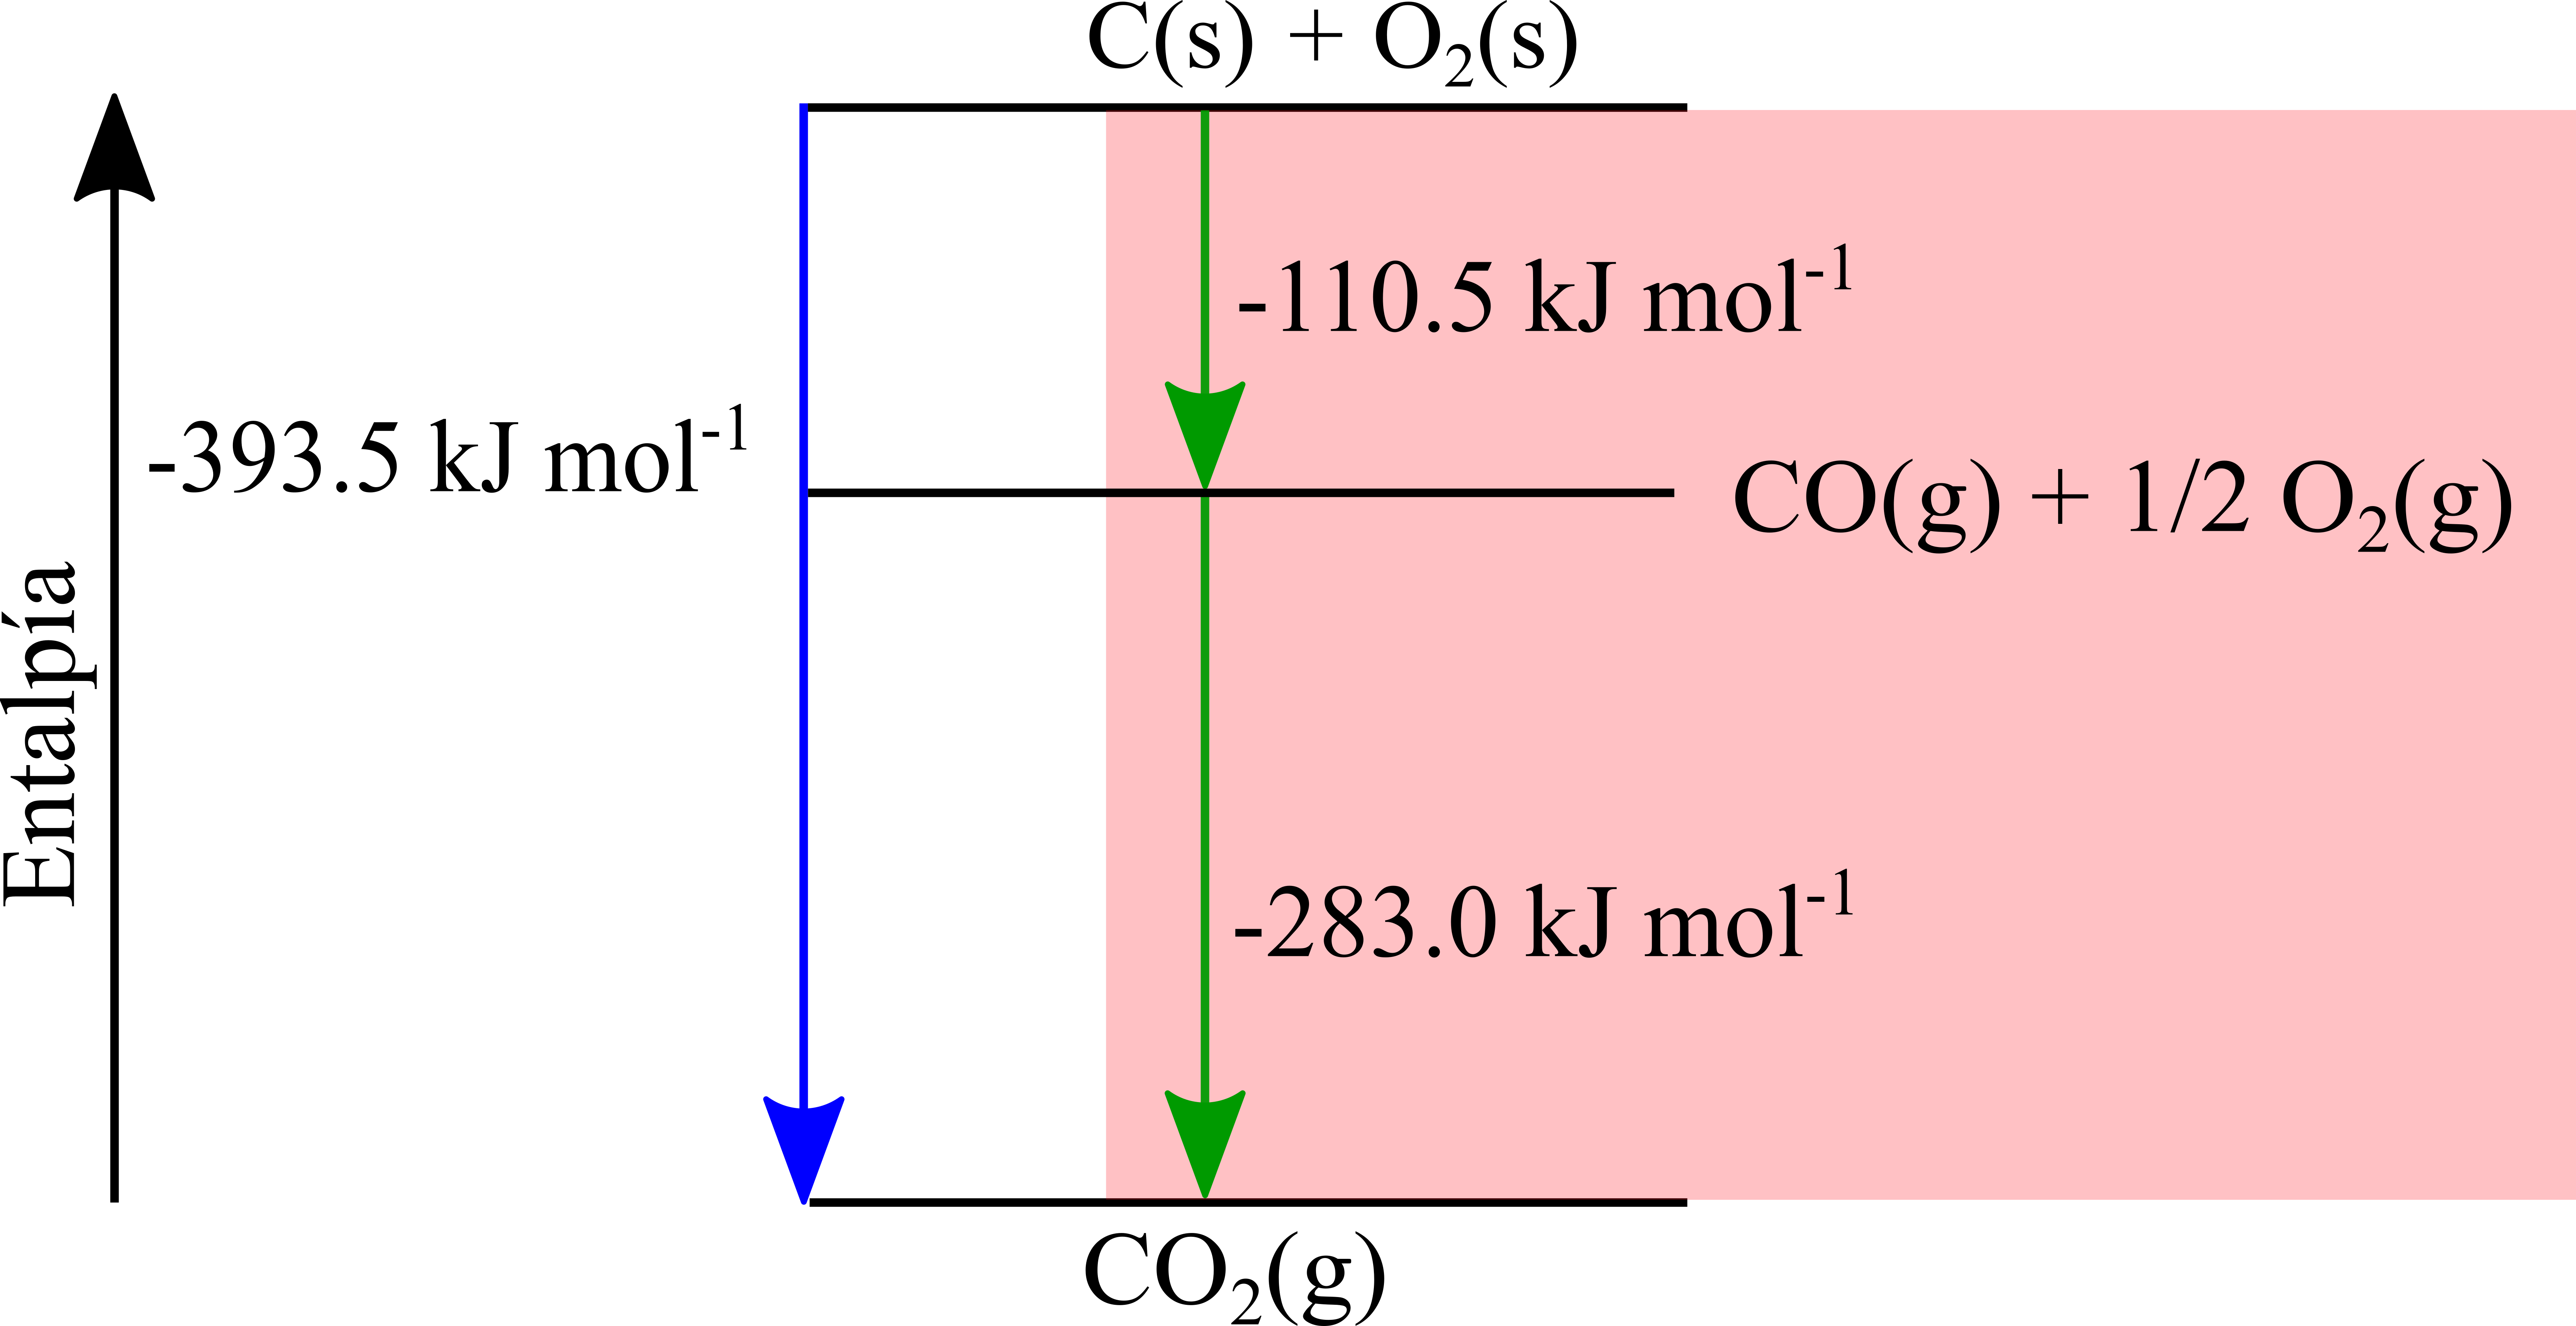
\includegraphics[scale=0.6]{graphs/CO.png}
\caption[Figura de la entalpía de formación de monóxido de carbono.]{Entalpía de formación de monóxido de carbono. El cambio de entalpía de la reacción total es igual a la suma de los cambios de entalpía de los dos pasos.}
\label{CO}
\end{center}
\end{figure}

\section{Química computacional}
Los métodos comentados en la sección \ref{sec:Hess}, permiten calcular los cambios de entalpía para una gran cantidad de reacciones (hay extensas tablas de entalpías de vaporización, entalpías de fusión y entalpías de combustión) \cite{NIST1998, Tajti2004, Nicolaides1996}. No obstante, también es posible cuantificar la entalpía de formación mediante cálculos \textit{ab initio} \cite{Lewars2016}.\\

La determinación de entalpías de formación por métodos computacionales es fundamental, porque sirve como información de entrada para multitud de simulaciones numéricas. Tal es la importancia, que se ha invertido un gran esfuerzo en la tabulación y refinamiento de \textit{JANAF}\cite{NIST1998}, \textit{CODATA}\cite{Cox1989}, \textit{Third Millenium}\cite{Goos1998} y \textit{Active Thermochemical Tables (ATcT)}\cite{Ruscic2004, Ruscic2005, Ruscic2005b}. Aunque la determinación experimental (principalmente mediante calorimetría) es el método más usado para obtener $\enthalpy*(f){}$, es a la vez, laborioso y consume mucho tiempo. Es claro que obtener $\enthalpy*(f){}$ experimental para todos los compuestos existentes es imposible y costoso. No obstante, ahora se acepta que la química teórica, ya sea de forma aislada o en conjunto con el experimento, pueda ofrecer un medio eficaz para obtener esta información.\\

La búsqueda del ``cielo químico'' en química computacional esta sujeto en gran medida, al tipo de metodología que sea capaz de predecir entalpías de formación con desviaciones menores a 4.184 kJ mol$^{-1}$ respecto al valor experimental. Por lo tanto, la precisión de cualquier $\enthalpy*(f){}$ depende del modelo químico aplicado y del tamaño del sistema molecular. Los métodos compuestos ofrecen una alternativa rentable a expensas de la precisión y consisten en una serie de optimizaciones de la geometría y cálculos de energía en un solo punto, con correcciones empíricas para superar las deficiencias cuando los métodos son comparados con entalpías de formación conocidas. Numerosos métodos se han usado en los últimos tiempos; los métodos CBS-x \cite{Montgomery2000, Ochterski1996} (x = QBB3 y APNO) y Gaussian-x \cite{Pople1989,Curtiss1990, Curtiss1991, Curtiss1998, Curtiss2007} (x = 1, 2, 3, 4), que son empleados en cálculos cinéticos y termodinámicos, siendo de gran relevancia para la termoquímica. 

Variantes del método G3, tales como G3B3 \cite{Baboul1999} y G3MP2 \cite{Curtiss1999} también son populares. El método G3 se emplea con frecuencia para la $\enthalpy*(f){}$ reportada por Burcat \textit{et al.} como parte de la base de datos \textit{Third Millenium}, con una incertidumbre de 8 kJ mol$^{-1}$. Los métodos ``estándar'' se han ajustado en numerosas ocasiones para remediar las dificultades percibidas con el objetivo de mejorar el coste computacional; un ejemplo de ello, son las variantes  de G4 \cite{Chan2010, Chan2011}, W1 \cite{Chan2012, Karton2012} y W3 \cite{Chan2013, Gruzman2009}. Para superar las grandes incertidumbres y errores en $\enthalpy*(f){}$ se emplea el método isodésmico, sin embargo, surge  un gran número de problemas al emplear este método porque se requieren entalpías de formación experimentales o métodos computacionales con un alto nivel de teoría para crear estas reacciones de trabajo hipotéticas;  los $\enthalpy*(f){}$ calculados dependen de la calidad de la reacción isodésmica (dado que no hay una única respuesta), además, el costo computacional se incrementa bastante. Pese a esto, los métodos computacionales pueden ofrecer excelentes resultados \cite{Simmie2015}.

\section{Métodos Gaussianos}

La clave de estos métodos es el uso de altos niveles de correlación y grandes conjuntos de bases. Esta serie comenzó en 1989 con \textit{Gaussian 1}, G1 \cite{Pople1989}, continuó con G2 (1991) \cite{Curtiss1991}, G3 (1998) \cite{Curtiss1998}, y G4 vio la publicación en 2007 \cite{Curtiss2007}. G1 y G2 están obsoletos. Los métodos Gaussianos de alta precisión más populares en la actualidad son probablemente G4 y G3 en conjunto de sus variantes más rápidas, G4(MP2) \cite{Curtiss2007a} y G3(MP2) \cite{Curtiss1999}. El uso continuo de G3 y G3(MP2) con G4 y G4(MP2) puede estar justificado por el deseo de comparar algunos trabajos actuales con resultados de métodos más antiguos. Para G3, la desviación absoluta media del experimento es de 4.7 kJ mol$^{-1}$, para G3(MP2)  es de 5.0 – 5.4 kJ mol$^{-1}$, es importante resaltar que G3(MP2) es de 7 a 8 veces más rápido que G3 \cite{Curtiss1998}. Para acelerar el método G4, sus pasos MP4 fueron reemplazados por MP2 y MP3 dando como resultado G4(MP2) y G4(MP3) \cite{Curtiss2007a, Lewars2016}. \\ Un cálculo G4, utiliza los siguientes pasos:
 
\begin{enumerate}
\item Obtención de la estructura de equilibrio en un nivel B3LYP/6-31G(2\textit{df,p}).
\item Especificación de las frecuencias armónicas.
\item Determinación de límite de energía Hartree-Fock.
\item Corrección de la energía.
\item Evaluación de la energía MP4/6-31G(\textit{d}), correcciones del paso anterior y combinación aditiva con el paso 3. 
\item Especificación de un nivel alto (HLC) con parámetros empíricos.
\item Obtención de la energía total a \textit{T} = 0 con una corrección en la energía de punto zero obtenida en el paso 2. 
\end{enumerate}

Estos siete pasos se utilizan para calcular una energía molecular como la suma de varias diferencias de energía y un incremento de energía empírica final (la ``corrección de nivel superior’’) en función del número de electrones apareados y no apareados. Debido a las correcciones de energía empírica en los métodos  gaussianos, no son completamente \textit{ab initio}, sino algo \textit{semiempíricos}, excepto cuando estas correcciones se anulan. Esta cancelación ocurre, por ejemplo, al calcular las afinidades de los protones como la diferencia de energía de las especies protonadas y no protonadas. Los métodos gaussianos, CBS y otros no mencionados aquí, son revisados  por Peterson, Feller y Dixon en el año 2012, con énfasis en termoquímica; estos autores reconocen una precisión química de 4 kJ mol$^{-1}$ como aceptable \cite{Peterson2012}. \\

\section{Métodos CBS}
En estos métodos se usa una extrapolación del conjunto de bases a un límite infinito (hasta el final). Hay tres métodos CBS básicos: CBS-4 (para extrapolación de cuarto orden), CBS-Q (para CI cuadrático) y CBS-APNO (para orbitales naturales de pares asintóticos, referidos a la extrapolación al límite establecido de base). Dichos métodos están disponibles en los programas \textit{Gaussian 94} y posteriores. CBS-4M puede manejar moléculas con hasta 19 átomos pesados. Los errores CBS-4M más típicos son (desviación absoluta media del experimento) 13.6 kJ mol$^{-1}$ \cite{Montgomery2000}. Hay una modificación de CBS-4M diseñada para disminuir la acumulación de errores con el aumento del tamaño molecular. CBS-QB3 puede manejar moléculas con hasta 13 átomos pesados y tiene una desviación media absoluta del experimento de 4.6 kJ mol$^{-1}$ \cite{Montgomery1999}. CBS-APNO puede manejar moléculas con hasta 7 átomos pesados y tiene una desviación absoluta media del experimento de 2.2 kJ mol$^{-1}$ \cite{Irikura1998}. Este conjunto de métodos implican esencialmente siete u ocho pasos \cite{Lewars2016}:

\begin{enumerate}
\item Una optimización de geometría (en el nivel HF/3–21G(*) o MP2/6–31G*, dependiendo del método CBS en particular).

\item Cálculo de ZPE a nivel de optimización.

\item Determinación de punto único de HF con un conjunto de bases muy grande (6–311 + G(3d2f,2df,p) o 6–311 + G(3d2f,2df,2p), dependiendo del método CBS).

\item Cálculo de punto único MP2 (base que depende del método CBS).

\item Extrapolación de un par de orbitales naturales para estimar el error debido al uso de un conjunto de bases finitas.

\item Determinación de energía MP4.

\item Para algunos métodos CBS, un cálculo de punto único QCISD(T).

\item Una o más correcciones empíricas, teniendo en cuenta el aspecto semiempírico de los métodos CBS. 

\end{enumerate}


\section{Comparacion entre métodos} 
En este trabajo nos concentraremos en los métodos de tipo gaussiano y CBS (en especial de tipo gaussiano), porque estos han sido los más utilizados, y por lo tanto, han acumulado una gran cantidad de resultados publicados, además de ser los más accesibles. Sin embargo, como ya mencionamos, existen otros métodos de alta precisión, como los procedimientos de Weizmann de Martin y de Oliveira, W1 y W2 \cite{Martin1999},  Boese \textit{et al.} W3 y W4 \cite{Boese2004} y las modificaciones más rápidas de estos como W2X y W3X-L de Chan y Radom \cite{Chan2015}, los cuales, al igual que los métodos CBS, se basan en la extrapolación de conjuntos de bases. El autor principal de esta revisión es el profesor K. A. Peterson de la Universidad Estatal de Washington; los métodos CBS provienen del grupo de investigación del profesor G. A. Petersson de la Universidad Wesleyana; ambos investigadores están activos en termoquímica cuántica computacional.\\

De los métodos de tipo gaussiano y CBS, para una alta precisión en moléculas muy pequeñas, CBS-APNO es la elección adecuada, y para moléculas "grandes", la elección recae en CBS-4M con la aceptación de la posibilidad de errores moderadamente grandes. Para moléculas de tamaño intermedio, la mejor elección es probablemente entre G4(MP2) y CBS-QB3. Recordemos que G4(MP2) es mucho más rápido que G4, con poca pérdida de precisión en la mayoría de los casos \cite{Lewars2016}.\\

\begin{comment}
En la tabla \ref{Fattahi-table} se muestra una comparación de los métodos gaussianos y un método CBS, usando 1,4-benzoquinona (p-benzoquinona, $O=C_{6}H_{4}=O$) al calcular la entalpía de formación por el método de atomización. Se debe tener en cuenta que el cálculo G4 tomó nueve veces más tiempo (160/18) que el G4 (MP2) y ambos dieron casi la misma entalpía de formación \cite{Lewars2016}. 

\begin{table}[H]
\begin{center}
\begin{tabular}{||l|c|c||}
\hline 
Método & $\Delta_{f}$H/(kJ mol$^{-1})$ & minutos/tiempo relativo \\ 
\hline 
G4 & -117.5 & 160/21 \\ 
\hline 
G4(MP2) & -118.5 & 18/2.4 \\ 
\hline 
G3 & -118.6 & 24/3.2 \\ 
\hline 
G3(MP2) & -120.0 & 7.5/1 \\ 
\hline 
CBS-QB3 & -115.9 & 16/2.1 \\ 
\hline 
\end{tabular} 
\end{center}
\caption[La entalpía de formación aceptada en la literatura es de -122. $\pm$ 3.8 kJ mol$^{-1}$ \cite{Fattahi2005}.]{Los primeros cuatro valores calculados experimentalmente están dentro de 1 kJ mol$^{-1}$, sin embargo, el valor CBS-QB3 es de 3 kJ mol$^{-1}$ y está por encima del mayor error estimado. No obstante, no se debe generalizar a partir de una muestra de un solo compuesto.}
\label{Fattahi-table}
\end{table}

\end{comment}

\section{Método de atomización} 

En química computacional hay tres enfoques principales que predicen entalpías de formación. 

\begin{enumerate}
\item Método de atomización.
\item Método de formación.
\item Método de reacciones isodésmicas.
\end{enumerate}

 
De los 3 enfoques anteriores, el método de atomización da mejores resultados, especialmente para moléculas orgánicas y es el más sencillo, porque se basa en la ruptura de enlaces de una molécula para obtener a sus átomos en fase gas\cite{Nicolaides1996}. A continuación se analizará el principio del método de atomización con la molécula de metanol. \\

La entalpía de atomización, $\Delta_{\mathrm{a}} H^{\circleddash}_{T}$ a \textit{T} = 0 \textit{ab initio}, del metanol es la diferencia de entalpía entre los átomos de la molécula y el metanol. Para calcular $\Delta_{\mathrm{f}}H^{\circleddash}_{0}$ se requiere la entalpía de formación a \textit{T} = 0 de los átomos de C, H y O y la entalpía de atomización a \textit{T} = 0 del metanol (ecuaciones \ref{eq:3.14} y \ref{eq:3.15}). Las entalpías de atomización del hidrógeno y el oxígeno se pueden calcular por un método \textit{ab initio}, pero no de forma fiable y precisa. Para mantener la coherencia, utilizaremos valores experimentales de las tres entalpías de atomización elementales, como recomiendan Nicolaides \textit{et al.}\cite{Nicolaides1996}. De la ecuación \ref{eq:3.16}, la entalpía de atomización \textit{T} = 0 del metanol es simplemente las suma de las entalpías \textit{ab initio} de los átomos que la constituyen menos la entalpía \textit{ab initio} corregida por ZPE del metanol:

\begin{equation}
	\Delta_{\mathrm{f}} H^{\circleddash}_{0}(\mathrm{CH_3OH}) + \Delta_{\mathrm{a}} H^{\circleddash}_{0} (\mathrm{CH_{3}OH}) = \Delta_{\mathrm{f}} H^{\circleddash}_{0} \mathrm{(C(^{3}P) + 4H(^{2}S) + O(^{3}S))}
\label{eq:3.14}
\end{equation}\\

\begin{equation}
	\Delta_{\mathrm{f}} H^{\circleddash}_{0}(\mathrm{CH_3OH}) = \Delta_{\mathrm{f}} H^{\circleddash}_{0} \mathrm{(C(^{3}P) + 4H(^{2}S) + O(^{3}S))} - \Delta_{\mathrm{f}} H^{\circleddash}_{0} \mathrm{(CH_3OH)}
\label{eq:3.15}
\end{equation}\\

\begin{equation}
	\Delta_{\mathrm{a}} H^{\circleddash}_{0}(\mathrm{CH_3OH)} = \Delta E^{total}_{0\mathrm{K}} \mathrm{(C(^{3}P) + 4H(^{2}S) + O(^{3}S))} - \Delta E^{total}_{0\mathrm{K}}(\mathrm{CH_3OH)}
\label{eq:3.16}
\end{equation}\\

\begin{figure}[H]
\begin{center}
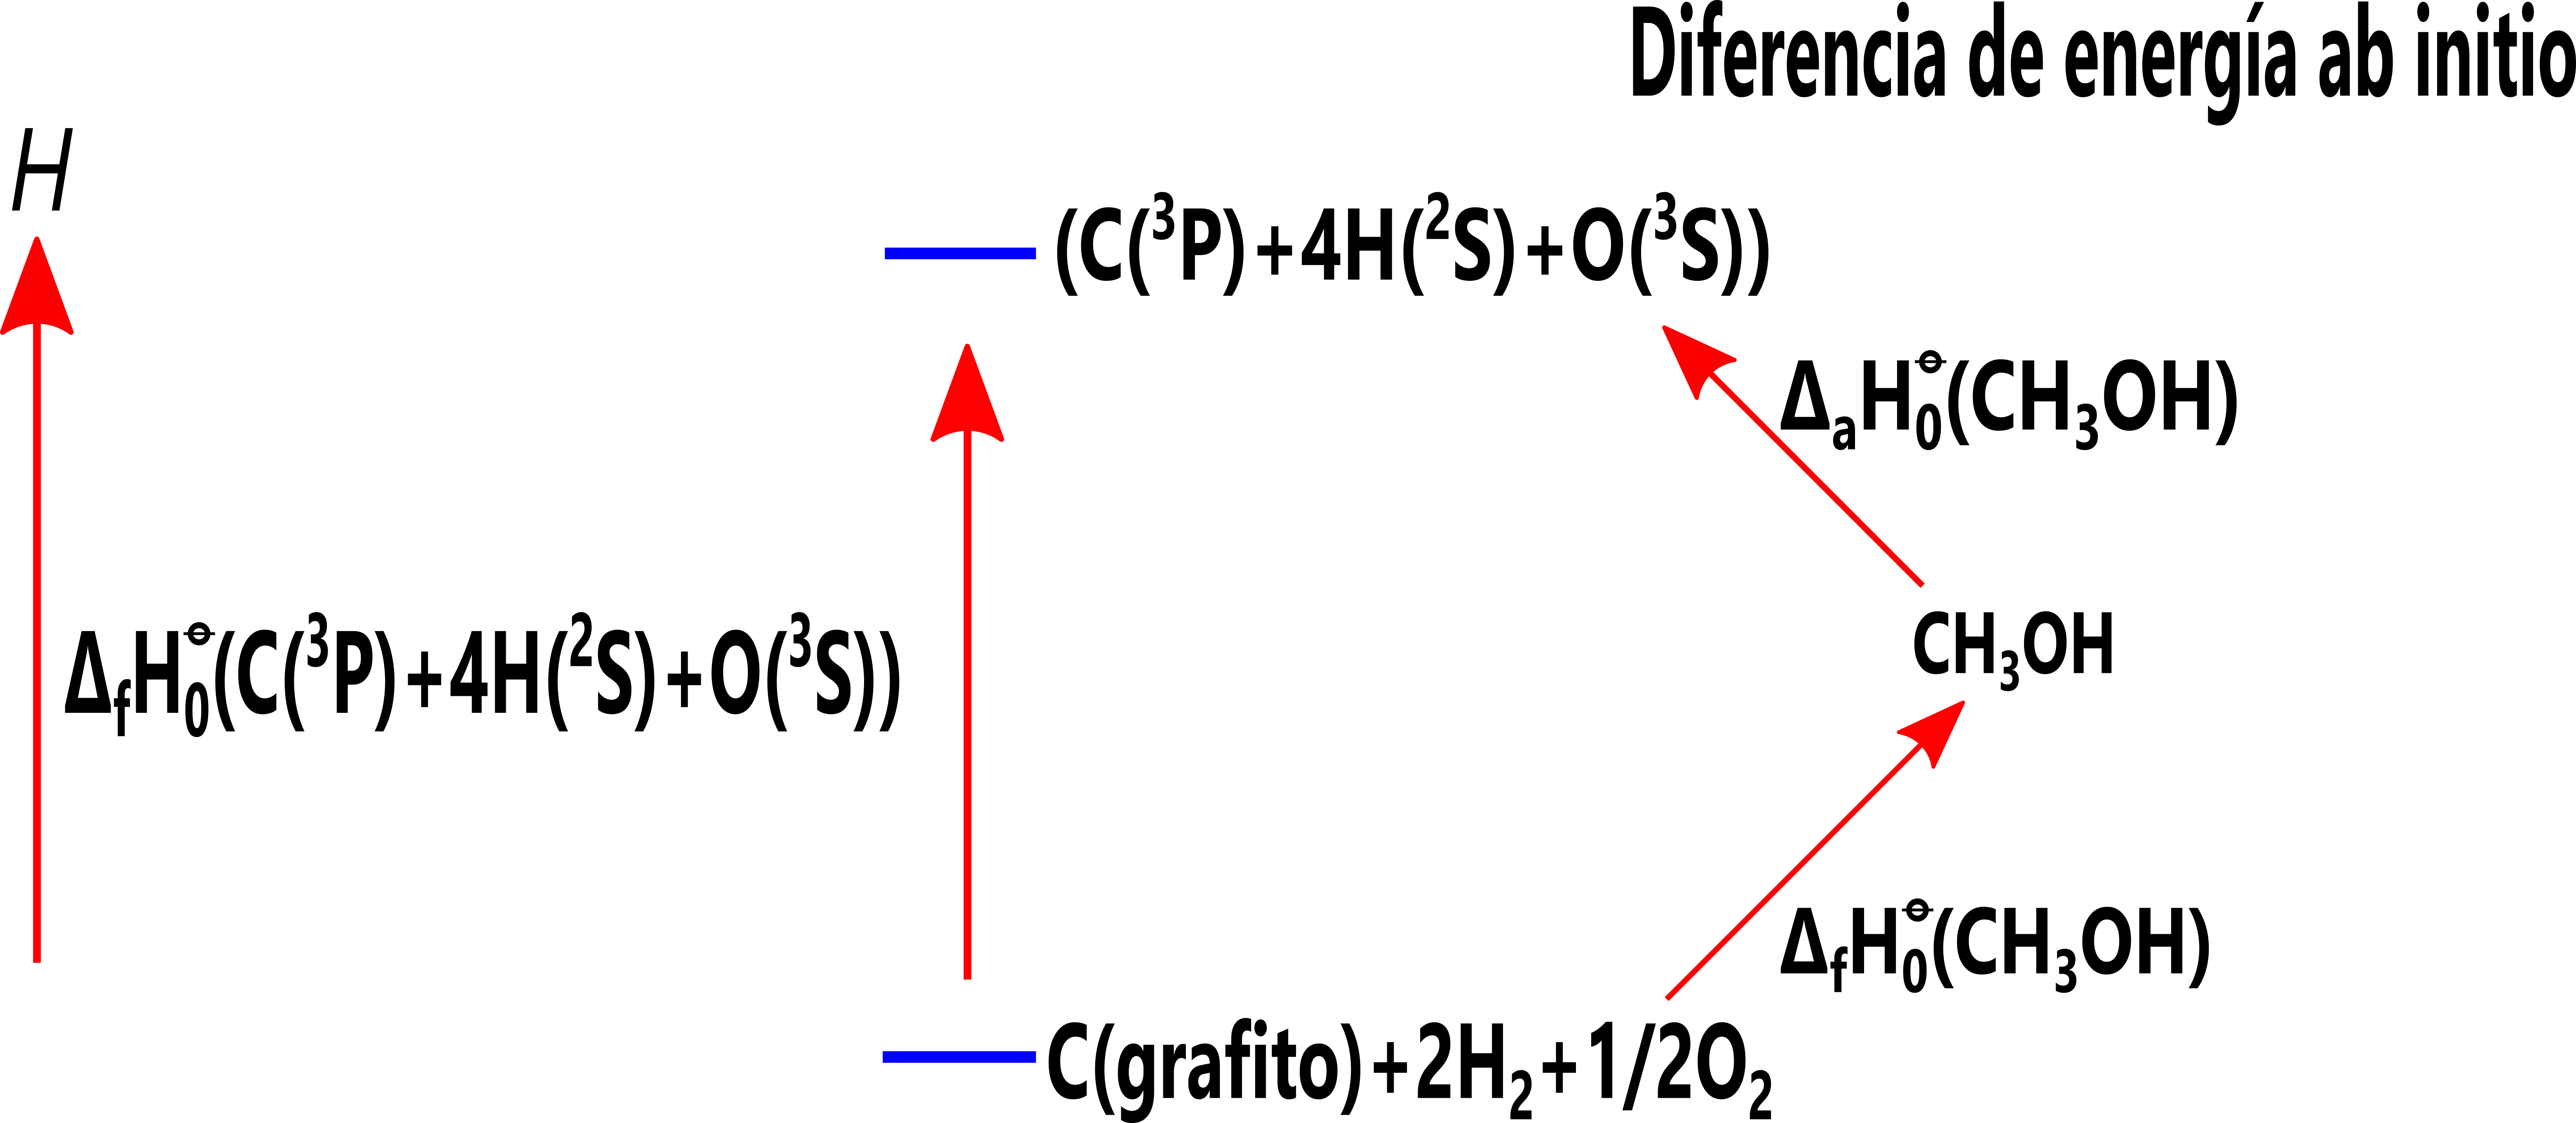
\includegraphics[scale=.6]{graphs/atomization-CH3OH.png}
	\caption[Figura de entalpía de atomización de metanol.]{El metanol se atomiza (conceptualmente) a \textit{T} = 0 en los átomos que lo constituyen, es decir,  carbono, hidrógeno y oxígeno (en sus estados electrónicos fundamentales). Además, los átomos de la molécula en sus estados estándar también son usados para formar dicha molécula. La entalpía de formación del metanol a \textit{T} = 0, $\Delta_{\mathrm{f}} H^{\circleddash}_{0}$(CH$_3$OH), se obtiene al igualar la energía necesaria para generar los átomos a través del metanol ($ \Delta_{\mathrm{f}} H^{\circleddash}_{0}$(CH$_3$OH) + $ \Delta_\mathrm{{a}} H^{\circleddash}_{0}$(CH$_3$OH)) a la energía para hacerlo directamente desde sus elementos en sus estados estándar \cite{Lewars2016}.}
\label{atm-metanol}
\end{center}
\end{figure}

Los valores experimentales de las entalpías de atomización de los átomos a \textit{T} = 0 de $\mathrm{(C(^{3}P) + 4H(^{2}S) + O(^{3}S))}$ se ilustran en la tabla \ref{Nicolaides-table}.

\begin{table}[H]
\begin{center}
\begin{tabular}{||c|c||}
\hline 
Átomo  & Entalpía experimental/(kJ mol$^{-1}$) \\ 
\hline 
\hline
C & 711.185 \\ 
\hline 
H & 216.03500 \\ 
\hline 
O & 246.7900 \\ 
\hline 
\end{tabular}
	\caption{Entalpías de formación experimentales reportadas por Nicolaides \textit{et al.} \cite{Nicolaides1996}.}
\label{Nicolaides-table}
\end{center}
\end{table}

Posteriormente, para calcular $\Delta_{\mathrm{a}} H^{\circleddash}_{0} \mathrm{(CH_3OH)}$ se usará la ecuación \ref{eq:3.16} que toma el valor de $\Delta E^{total}_{0\mathrm{K}}$ para los átomos de  C, H, y O. En lugar del método G2 que fue empleado por Nicolaides \textit{et al.} \cite{Nicolaides1996}, usaremos el método G4 de \textit{Gaussian09}. Los valores obtenidos para cada átomo y su respectiva molécula a \textit{T} = 0 se muestran en la tabla \ref{G4-table}.\\


\begin{table}[H]
\begin{center}
\begin{tabular}{||c|c||}
\hline 
	Átomos  & Entalpías G4 a \textit{T} = 0  (hartrees) \\ 
\hline
\hline 
C & -37.834170 \\ 
\hline 
H & -0.501420 \\ 
\hline 
O & -75.045500 \\ 
\hline 
CH$_{3}$OH & -115.651767 \\
\hline
\end{tabular}
	\caption{Entalpías de formación a \textit{T} = 0 obtenidas por el método G4 de Gaussian09.}
\label{G4-table}
\end{center}
\end{table}


El valor de metanol de $-115.651767$ h podría llamarse el ``cero absoluto'' de la entalpía del metanol, es decir, la entalpía relativa a la de los núcleos disociados y electrones. Esta entalpía absoluta se utilizará en el cálculo de la entalpía de formación. De la ecuación \ref{eq:3.16} es posible calcular la energía de atomización de metanol a \textit{T} = 0:

\begin{multline}
	\Delta_{\mathrm{a}} H^{\circleddash}_{0}\;\mathrm{(CH_3OH)} = -37.834170\;\mathrm{h} + 4(-0.501420)\;\mathrm{h}-75.045500\;\mathrm{h}-(-115.651767)\;\mathrm{h} =...\\
	...= (0.766417\;\mathrm{h})(2625.5\;\mathrm{kJ\;mol^{-1}}) = 2012.227\;\mathrm{kJ\;mol^{-1}}
\label{eq:3.17}
\end{multline}\\

De la ecuación \ref{eq:3.14} la entalpía de formación a \textit{T} = 0 de metanol es:\\

\begin{multline}
	\Delta_{\mathrm{f}} H^{\circleddash}_{0}\mathrm{(CH_3OH)} = 711.185\;\mathrm{kJ\;mol^{-1}} + 4(216.03500)\;\mathrm{kJ\;mol^{-1}} +... \\...\; 246.7900\;\mathrm{kJ\;mol^{-1}}- 2012.227\;\mathrm{kJ\;mol^{-1} = -190.112\;kJ\;mol^{-1}}
\label{eq:3.18}
\end{multline}\\

Nicolaides \textit{et al.} \cite{Nicolaides1996} reportaron un valor de 195.7 kJ mol$^{-1}$ a \textit{T} = 0 mediante el método de atomización junto con los valores experimentales, que son 190.7 kJ mol$^{-1}$ y 189.8 kJ mol$^{-1}$, que concuerdan con el valor G4 calculado aquí. Cualquier inexactitud en la energía de atomización calculada, se mostrará en la entalpía de formación, y solo un buen método de alta precisión puede mitigar este error de manera confiable. Para ajustar la entalpía de formación de \textit{T} = 0 a \textit{T} = 298 K, debemos agregar dicho valor y restar los aumentos correspondientes para los elementos en sus estados estándar. El valor para el metanol es la diferencia de las dos cantidades G4 proporcionadas en el archivo de salida de Gaussian. El aumento de la entalpía del metanol al pasar de \textit{T} = 0 a \textit{T} = 298 K es:


\begin{equation}
	\Delta \Delta H^{\circleddash}(\mathrm{CH_3OH}) = \mathrm{G4}\;\textrm{Entalpía} - \mathrm{G4} \;(0\mathrm{K})
\label{eq:3.19}
\end{equation}\\

\begin{multline}
	\Delta \Delta H^{\circleddash}\mathrm{(CH_3OH)} = -115.647489\;\mathrm{h} - (-115.651767\;\mathrm{h})\; =...\\
	...= (0.004278\;\mathrm{h})(2625.5\;\mathrm{kJ\;mol^{-1})} = 11.23188\;\mathrm{kJ\;mol^{-1}}
\label{eq:3.20}
\end{multline}\\

Las entalpías experimentales de los respectivos elementos también es reportada por Nicolaides \textit{et al.}\cite{Nicolaides1996} en kJ mol$^{-1}$, véase la tabla \ref{Nicolaides-exp-table}.

\begin{table}[H]
\begin{center}
\begin{tabular}{||c|c||}
\hline 
	Átomos  & Entalpía experimental/($\mathrm{kJ\;mol^{-1}}$) \\ 
\hline 
C(grafito) & 1.05100 \\ 
\hline 
H$_{2}$ & 8.46700 \\ 
\hline 
O$_{2}$ & 8.67000 \\ 
\hline 
\end{tabular}
	\caption{Entalpías experimentales de los elementos reportadas por Nicolaides \textit{et al.}\cite{Nicolaides1996}.}
\label{Nicolaides-exp-table}
\end{center}
\end{table}

Ahora, para ajustar la entalpía de formación a un estado estándar, sumamos el aumento de entalpía del metanol al pasar de \textit{T} = 0 a \textit{T} = 298 K y restamos los aumentos correspondientes de los elementos en sus estados estándar.

\begin{multline}
	\enthalpy*(f){} \mathrm{(CH_3OH)} = \Delta_{\mathrm{f}} H_{0}^{\circleddash}\mathrm{(CH_{3}OH)} + \Delta \Delta H^{\circleddash} \mathrm{(CH_{3}OH)} \\ - (\Delta \Delta H^{\circleddash} \mathrm{(C)} + 2 \Delta \Delta H^{\circleddash}(\mathrm{H_{2}}) + \frac{1}{2} \Delta \Delta \mathrm{H}^{\circleddash}\mathrm{(O_{2}))}
\label{eq:3.21}
\end{multline}\\

\begin{multline}
	\enthalpy*(f){} \mathrm{(CH_3OH)} = -190.112\;\mathrm{kJ\;mol^{-1}} + 11.23188\;\mathrm{kJ\;mol^{-1}}  \\ - (1.05100 + 2(8.467000) + \frac{1}{2} (8.6700))\;\mathrm{kJ\;mol^{-1}}
\label{eq:3.22}
\end{multline}\\

\begin{equation}
	\enthalpy*(f){} \mathrm{(CH_3OH)} = -201.20\;\mathrm{kJ\;mol^{-1}}
\label{eq:3.23}
\end{equation}\\

El valor experimental a \textit{T} = 298 K aceptado es de -205 $\pm$ 10 kJ mol$^{-1}$\cite{Afeefy2009}. Por lo tanto, la cifra calculada está dentro del error experimental esperado \cite{Lewars2016}.


\section{Relaciones Generales de Termodinámica Estadística}

Algunos métodos computacionales, particularmente las técnicas \textit{ab initio}, producen información molecular detallada pero no información termodinámica directamente. Se necesitan más cálculos para generar cantidades como la entropía molar estándar (S°), la capacidad calorífica (C$_{p}$) y el cambio de entalpía \textit{[H°(T)-H°(0)]}. En algunos cálculos \textit{ab initio}, los resultados ni siquiera corresponden a las propiedades a temperatura de cero absoluto y siempre deben corregirse. Estas correcciones se basan en la Termodinámica Estadística, en dependencia de la función de partición molecular, $Q$. La función de partición se usa no solo para predicciones teóricas, sino también para generar la mayoría de las tablas termoquímicas publicadas. 

Los modelos \textit{ab initio} también  utilizan la aproximación Born-Oppenheimer. La base física de la aproximación de Born-Oppenheimer es que los núcleos son mucho más masivos que los electrones, por lo tanto, se mueven lentamente en relación con los electrones. En consecuencia, se puede considerar que los electrones se mueven en un campo producido por los núcleos fijados en alguna separación internuclear. Las energías resultantes son correctas para una molécula hipotética que no vibra. Aunque los osciladores pueden estar en reposo en la mecánica clásica, los osciladores reales (mecánica cuántica) siempre están en movimiento. El pequeño movimiento residual a la temperatura de cero absoluto es la energía vibracional de punto cero, abreviada como ZPVE o ZPE. Para un oscilador armónico simple, el ZPE es igual a la mitad de la frecuencia vibracional. Aunque todas las vibraciones moleculares reales son al menos ligeramente anarmónicas, por lo general se aproximan como armónicas. Así pues, la ZPE de una molécula puede calcularse como la mitad de la suma de las frecuencias vibracionales. En la ecuación \ref{eq:3.24}, $N$ es el número de átomos en la molécula, $\nu _{i}$ son las frecuencias vibracionales fundamentales. Hay vibraciones $3N-6$ en una molécula no lineal y $3N-5$ en una molécula lineal; la ecuación \ref{eq:3.24} es para el caso no lineal. El ZPE debe agregarse a la energía \textit{ab initio} para obtener una energía correspondiente a \textit{T} = 0.

\begin{equation}
ZPE = \frac{1}{2} \sum_{i=1}^{3N-6} \nu_{i}
\label{eq:3.24}
\end{equation}\\

En la práctica, la corrección ZPE se complica un poco debido a que las
frecuencias vibracionales \textit{ab initio} a menudo tienen un error de $+5\%$ a $+10\%$. Para compensar este error, las frecuencias calculadas generalmente se multiplican por factores de escala empíricos. Las recomendaciones más recientes son las de Scott \textit{et al.} \cite{Scott1996}. Por ejemplo, sugieren escalar las frecuencias HF/6-31G* en 0.8953 para predecir espectros de vibración (es decir, frecuencias fundamentales), en 0.9135 para el cálculo de ZPE, en 0.8905 para predecir diferencias de entalpía $[H^{\circ}(298.15) - H^{\circ}(0)]$.\\

La Termodinámica Estadística pretende incluir los métodos utilizados para convertir los niveles de energía molecular en propiedades macroscópicas, especialmente entalpías, entropías y capacidades caloríficas. Los niveles de energía molecular surgen de la traslación molecular (es decir, el movimiento a través del espacio), la rotación, la vibración y la excitación electrónica. Esta información constituye la espectroscopia de la molécula de interés y puede obtenerse experimentalmente o mediante cálculos \textit{ab initio} \cite{Irikura1998}. \\

\subsection{Función de partición}

Los niveles de energía molecular $\varepsilon_{i}$ se utilizan para calcular la función de partición molecular, generalmente denotada por el símbolo $Q$, como se muestra en la ecuación \ref{eq:3.25} (se extiende sobre todos los niveles de energía). 

\begin{equation}
Q(T) =  \sum_{i=1} e^{-\frac{\varepsilon_{i}}{kT}}
\label{eq:3.25}
\end{equation}\\

Sin embargo, para temperaturas muy altas donde las moléculas se vuelven inestables, la extensión de la suma puede ser ambigua. Los datos termoquímicos tabulados deben utilizarse con precaución en tales condiciones porque los valores (1) pueden depender en gran medida del procedimiento de energía adoptado y (2) pueden desviarse implícitamente del modelo de gas ideal. Normalmente, uno elige el nivel de energía más bajo para que sea el cero de energía, de modo que ningún nivel se encuentre en energías negativas. De la ecuación \ref{eq:3.25} se deduce que las mayores contribuciones para $Q$ provienen de los niveles de energía más bajos. Por el contrario, los niveles que se encuentran muy por encima de \textit{kT} (207 cm$^{-1}$ a temperatura ambiente) tienen solo un efecto menor sobre $Q$ y sus cantidades termodinámicas derivadas \cite{Irikura1998}.\\

\subsection{Funciones termodinámicas}

Dada la función de partición, se pueden calcular las funciones termodinámicas habituales. No obstante, aquí solo usaremos las ecuaciones que permiten calcular la diferencia relativa de entalpía, véase la ecuación de Kirchhoff (ecuación \ref{eq:3.26}) \cite{Irikura1998}.

\begin{equation}
H(T)-H(0) = \int_{0} ^{T} C_{p} dT = \frac{RT^{2}}{Q} \frac{\partial Q}{\partial T} + RT
\label{eq:3.26}
\end{equation}

\subsection{Cálculos prácticos}

Casi nunca se dispone de un conjunto completo de niveles de energía molecular. Para
simplificar el problema, se suele adoptar un modelo en el que la traslación, la rotación, la vibración y la excitación electrónica están desacopladas. En otras palabras, se asume que la aproximación de los diferentes tipos de movimiento no se afectan entre sí y no se mezclan. Esto conduce  a separar $Q$ en cuatro factores que corresponden a funciones de partición separadas para traslación, rotación, vibración y excitación electrónica. Esto se muestra en la ecuación \ref{eq:3.27}.

\begin{equation}
Q = Q_{tras}Q_{rot}Q_{vib}Q_{elec}
\label{eq:3.27}
\end{equation}\\

Cuando se consideran los estados electrónicamente excitados, a menudo se supone que
los espectros de traslación, rotación y vibración del estado excitado son los mismos que los del estado electrónico fundamental. Esto es conveniente cuando no hay otra información disponible. Además, si el estado excitado se encuentra muy por encima de \textit{kT}, los resultados finales no serán sensibles a tales detalles \cite{Irikura1998}. \\


\subsection{Función de partición traslacional}

$Q_{tras}$ debe calcularse a partir de una suma de todos los niveles de
energía de traslación que están disponibles para una molécula confinada en una caja
cúbica de volumen \textit{V = RT/p} (volumen molar de un gas ideal a temperatura \textit{T} y presión $p$).Esto rara vez se hace. En cambio, la suma se aproxima como una integral para obtener la ecuación \ref{eq:3.28}. Esta aproximación es buena siempre que $m^{3/2}/T^{5/2}$ $p^{-1}$ $\gg$ $h^{3}(2\pi)^{-3/2}k^{-5/2}$. Cuando $p$ = 1 bar, esta condición se cumple para moléculas suficientemente pesadas, $m$ (en uma) $\gg$ $11.4 T^{-5/3}$ y para temperaturas suficientemente altas, \textit{T} $\gg$ $4.31 m^{-3/5}$. Afortunadamente, esto cubre las condiciones de interés químico. Para un gas ideal monoatómico, no hay movimiento vibratorio o rotacional \cite{Irikura1998}.\\

\begin{equation}
[H(T)-H(0)]_{tras} = \frac{3}{2} RT
\label{eq:3.28}
\end{equation}\\

\newpage

\subsection{Función de partición rotacional}

La rotación libre de una molécula rígida también está cuantizada (el momento angular y su proyección son múltiplos enteros de $h/2\pi$), por lo que la energía de rotación está restringida a ciertos niveles discretos. Los espectros de rotación se caracterizan por las constantes $A, B, C$, donde $A \equiv$ $h/(8\pi^{2}I_{A}$) y lo mismo para $B$ y $C$. Las cantidades $I_{A,B,C}$ son los momentos principales de inercia de la molécula, con la convención $I_{A} \leq I_{B} \leq I_{C}$ (o $A \geq B \geq C$). Muchos programas, incluidos los paquetes \textit{ab initio}, informan las constantes de rotación cuando se les proporciona una geometría molecular. Los momentos también se pueden calcular manualmente como los valores propios del tensor de inercia, que tiene elementos como $I_{xy} = - \sum m_{i}x_{i}y_{i}$ y $I_{xx} = + \sum m_{i}x_{i}(y_{i}^{2}+z_{i}^{2})$, donde el índice $i$ recorre todos los átomos en la molécula y el origen de coordenadas está en el centro de masa. Las moléculas lineales $(I_{A} = 0)$ se describen mediante una sola constante de rotación $B$, y no solo por el momento de inercia, $I$. Afortunadamente, a temperaturas lo suficientemente altas ($kT \gg hA$), la suma se puede reemplazar por una integral como lo es para la traslación. En el caso general, la función de partición rotacional viene dada por la ecuación \ref{eq:3.29}. Para moléculas lineales, se debe usar la ecuación \ref{eq:3.30} en su lugar \cite{Irikura1998}.


\begin{equation}
[H(T)-H(0)]_{rot} = \frac{3}{2} RT
\label{eq:3.29}
\end{equation}


\begin{equation}
[H(T)-H(0)]_{rot}^{lineal} =  RT
\label{eq:3.30}
\end{equation}

\newpage

\subsection{Función de partición vibracional}

Para completar el modelo simple de rotor rígido/oscilador armónico (RROA), se deben
considerar las vibraciones moleculares. Como se indica en la discusión de ZPE (ecuación
\ref{eq:3.24}), una molécula que contiene $N$ átomos tiene $3N-6$ frecuencias vibratorias o $3N-5$ para moléculas lineales. Las función de partición para la entalpía está dada por la ecuación \ref{eq:3.31} \cite{Irikura1998}.

\begin{equation}
[H(T)-H(0)]_{vib}=RT \sum_i \left(\frac{h\nu_i}{kT}\right)\left(\frac{e^{\frac{-h\nu_i}{kT}}}{1-e^{\frac{-h\nu_i}{kT}}}\right)
\label{eq:3.31}
\end{equation}

\subsection{Función de partición electrónica}

Aunque es posible que no tengan excitación electrónica a baja temperatura estados, algunas moléculas tienen estados fundamentales electrónicos degenerados. Los radicales libres son un ejemplo común. Pueden tener electrones desapareados en sus estados básicos electrónicos y un espín electrónico neto de $S = n_{desapareado}/2$, donde $n_{desapareado}$ es el número de electrones desapareados. La multiplicidad, o degeneración $g$, de tal estado es $g = (2S+1)$. El uso de números de degeneración equivale a un recuento explícito de todos los estados, incluidos los degenerados. Por lo tanto, $Q_{elec} = g$ es una constante y solo afecta la entropía \cite{Irikura1998}.\\


\subsection{Cálculo de entalpía mediante Termodinámica Estadística}

Para calcular la entalpía se usan las ecuaciones \ref{eq:3.28}, \ref{eq:3.29}, \ref{eq:3.31} y \ref{eq:3.31}. Esto es $[H(298.15)-H(0)] = [H(T)-H(0)]_{vib}+[H(T)-H(0)]_{rot}+[H(T)-H(0)]_{tras}$. La contribución electrónica es ignorada (es decir, la función de partición correspondiente se establece en la unidad). Por otra parte, es posible remplazar la diferencia de las dos cantidades Gn o CBS proporcionadas en el resumen termoquímico  implementado en \textit{Gaussian} por el valor de la entalpía (energía interna) a partir de su función de partición \cite{Irikura1998}.


\section{Aproximación de Nicolaides}

 
Nicolaides \textit{et al.} en 1996, publicaron un artículo en el que intentaron corregir los posibles errores cuando existen rotores internos en moléculas. Por ejemplo, para el caso de la molécula de tolueno, el metilo que esta unido al anillo aromático puede estar girando, en consecuencia, es una mala idea usar la aproximación de rotor rígido/oscilador armónico, donde tendríamos un rotor rígido (en un rotor rígido la distancias relativas entre todas las partículas siempre es constante). Cuando una molécula gira o rota, pensaríamos que su geometría y distancias entre sus átomos nunca va a cambiar (ese es un error que se observa en la molécula de tolueno, porque el metilo rota de forma independiente). Y cuando suponemos a la molécula como un rotor rígido, estamos suponiendo que el metilo no rota, porque si rotase, la distancia relativa de los hidrógenos del metilo a los hidrógenos del anillo aromático cambiaría. Por lo tanto, ya no se cumpliría la definición de rotor rígido. No obstante, pensar en rotores rígidos, simplifica el problema matemático cuando se intenta calcular la función de partición, pero puede darnos errores con moléculas que contienen rotores internos. Es así, que se propone tratar a las rotaciones internas como rotores libres cuando las frecuencias vibraciones de las moléculas son menores a 260 cm$^{-1}$ y en su lugar utilizar $\frac{1}{2}$ de \textit{RT} para la contribución vibracional por cada frecuencia que sea menor a 260 cm$^{-1}$ \cite{Nicolaides1996}. Cuando esto no se cumpla, será necesario utilizar la aproximación de rotor rigido/oscilador armónico. Además, se debe añadir un \textit{RT} adicional a la energía interna para convertir a la energía en entalpía (el llamado término \textit{pV}). La ecuación general para el cálculo de la entalpía (energía interna) tendrá la siguiente forma, obsérvese la ecuación \ref{eq:3.32}.

\begin{equation}
[H(298.15)-H(0)] = [H(T)-H(0)]_{vib}+[H(T)-H(0)]_{rot}+[H(T)-H(0)]_{tras} + pV
\label{eq:3.32}
\end{equation}

\newpage

\section{Hardware y software}

Actualmente, las computadoras pueden realizar cálculos y tomar decisiones lógicas con una rapidez difícil de imaginar 
(miles de millones de cálculos en un segundo), más de lo que un humano podría realizar en toda su vida. 
Las computadoras procesan datos, bajo el control de un conjunto de instrucciones conocidas como programas de computadora. 
Estos programas guían a la computadora a través de conjuntos ordenados de acciones especificadas por gente conocida como programadores. 
A los programas que se ejecutan en una computadora se les denomina \textit{software}. A las partes de una computadora que consisten en varios dispositivos se les conoce como \textit{hardware} (teclado, pantalla, ratón, discos duros, memoria, unidades de procesamiento) \cite{Deitel2014}. 

\section{Lenguajes}

Los programadores escriben instrucciones en diversos lenguajes de programación, 
algunos de los cuales los comprende directamente la computadora, mientras que otros requieren pasos intermedios de traducción.

\subsection{Lenguajes máquina}
Cualquier computadora puede entender de manera directa sólo su propio lenguaje máquina (también conocido como código máquina), 
el cual se define según su diseño de \textit{hardware}. Por lo general, los lenguajes máquina consisten en cadenas de números (que finalmente se reducen a 1s y 0s). 
Dichos lenguajes son difíciles de comprender para los humanos.

\subsection{Lenguajes ensambladores}
La programación en lenguaje máquina era demasiado lenta y tediosa para la mayoría de los programadores. 
Por lo tanto, empezaron a utilizar abreviaturas del inglés para representar las operaciones elementales. 
Estas abreviaturas formaron la base de los lenguajes ensambladores. Se desarrollaron programas traductores conocidos como ensambladores para convertir los programas que se encontraban en lenguaje ensamblador a lenguaje máquina.
 Aunque el código en lenguaje ensamblador es más claro para los humanos, las computadoras no lo pueden entender sino hasta que se traduce en lenguaje máquina.

\subsection{Lenguajes de alto nivel}
Para agilizar el proceso de programación se desarrollaron los lenguajes de alto nivel, en donde podían escribirse instrucciones individuales 
para realizar tareas importantes. Los lenguajes de alto nivel, como C++, Java, C y Visual Basic nos permiten escribir instrucciones que son muy similares al inglés y 
contienen expresiones matemáticas de uso común. Los programas traductores llamados compiladores convierten los programas que se encuentran en lenguaje de alto nivel a programas en lenguaje máquina. 
El proceso de compilación de un programa escrito en lenguaje de alto nivel a un lenguaje máquina puede tardar un tiempo considerable en la computadora. Los programas intérpretes se desarrollaron para ejecutar programas en lenguaje de alto nivel de manera directa (sin el retraso de la compilación), aunque con mayor lentitud de la que se ejecutan los programas compilados. Los lenguajes de secuencias de comandos, como los populares lenguajes JavaScript y PHP para Web, son procesados por intérpretes \cite{Deitel2014}.

\section{Una breve introducción a C++}
Existe una gran cantidad de lenguajes de programación para escribir \textit{software} (un ejemplo muy conocido es C++, el cual fue desarrollado por Bjarne Stroustrup en 1979, en los laboratorios Bell). Si uno de estos lenguajes de programación fuera el más adecuado para todos los propósitos, entonces se esperaría que todos usaran este lenguaje, y todos los demás lenguajes eventualmente quedarían obsoletos. Esto, sin embargo, no es el caso. A continuación, se explicará por qué C++ es un lenguaje de programación adecuado para aplicaciones científicas y por qué no es la única opción \cite{Pitt2017}.

\subsection{Alcance de C++ en el ámbito científico}

 En el campo de la programación científica, se utilizan muchos lenguajes y la mayoría de los científicos optan por Matlab, C/C++ o Fortran. La primera y más convincente razón para usar C++ (así como C y Fortran) es porque es rápido. Es decir, con una programación y optimizaciones cuidadosas, un programa se puede compilar en código de máquina que puede usar todo el poder del \textit{hardware} disponible. Muchos lenguajes de secuencias de comandos (como Matlab y Python) son lenguajes ensambladores (el código que se escribe, se traduce a código de máquina en tiempo de ejecución). Otros lenguajes (como Java y C) se compilan a la mitad, en un código de bytes independiente del \textit{hardware} que luego se interpreta en tiempo de ejecución. La interpretación del tiempo de ejecución significa que parte de la potencia de la computadora se gasta en el proceso de conversión y también que es más difícil aplicar optimizaciones. Hoy en día, las implementaciones de Matlab, Python y Java utilizan trucos inteligentes como el almacenamiento en memoria caché de los pasos de compilación y la compilación justo a tiempo para que los programas se ejecuten más rápido. No obstante, estos trucos requieren un esfuerzo computacional, por lo tanto, es posible que estos lenguajes no utilicen completamente el poder de todo el \textit{hardware}. Una segunda razón para usar C++ es que hay una gran cantidad de bibliotecas numéricas para computación científica en C++ y lenguajes relacionados. Muchos algoritmos numéricos se establecieron en la década de 1950 y luego se incorporaron a las bibliotecas de \textit{software} (como EISPACK y LINPACK) en la década de 1970. Si se optara por escribir código utilizando \textit{software} bien establecido y probado, entonces se está construyendo sobre décadas de experiencia y mejora. Una tercera razón para elegir escribir código en C++ es que existe una amplia gama de herramientas comerciales y de código abierto que lo respaldan. En contraste, si estuviéramos distribuyendo programas de Matlab, se necesitaría tener Matlab y una licencia instalada porque es un producto propietario. Hay productos similares de código abierto (como GNU Octave), pero no existe garantía de que un programa de Matlab produzca la misma respuesta cuando se ejecute. En Octave, debido a que es de código cerrado, el significado de un programa puede cambiar entre versiones de Matlab. Por ejemplo, cuando se introdujo la compilación justo a tiempo en Matlab 7, la semántica operativa del lenguaje cambió sutilmente. Esto significa que una pequeña minoría de los programas de Matlab que se sabía que funcionaban bien con una versión de Matlab podría producir resultados incorrectos, errores o advertencias en otra versión. Una cuarta razón para elegir C++ es que tiene un modelo de gestión de memoria flexible. En un lenguaje como Java, parte de la memoria del sistema se usa en la interpretación y se usa un recolector de basura para ordenar la memoria que ya se no está usando, por lo que es posible que no se pueda predecir cuánta memoria va a necesitar un programa. En C++ podemos hacer esta predicción, pero es un arma de doble filo porque también se es responsable de que la memoria se administre correctamente. Una razón final para programar en C++ es que es un lenguaje orientado a objetos \cite{Pitt2017}. 

\subsection{C++ y la programación orientado a objetos}

C ++ es un lenguaje ``orientado a objetos''. ¿Qué distingue a un lenguaje que está orientado a objetos de uno que no lo está? Fundamentalmente, que la unidad básica del lenguaje es un objeto o clase, una entidad que reune funcionalidad y datos relacionados. Algunos conceptos relacionados con la programación orientación a objetos son:

\begin{itemize}

\item \textbf{Modularidad}. Todos los datos de un objeto en particular, y las operaciones que realizamos en este objeto, se guardan en uno o dos archivos y se pueden trabajar en forma independiente.
\item \textbf{Abstracción}. Las características esenciales y la funcionalidad de una clase se colocan en un solo lugar y los detalles de cómo funcionan no son importantes para el usuario de la clase. Por ejemplo, si se está utilizando una biblioteca de sistema lineal para resolver ecuaciones matriciales, no se debería necesitar conocer los detalles precisos de cómo se disponen las matrices en la memoria o el orden exacto en que un solucionador numérico realiza sus operaciones. Solo se debe saber cómo usar la funcionalidad de la biblioteca. 

\newpage

\item \textbf{Encapsulación}. La implementación de un objeto se mantiene oculta para el usuario de la clase. No se trata únicamente de claridad (abstrayendo los detalles). Es necesario evitar que el usuario modifique accidentalmente el funcionamiento interno de, por ejemplo, un solucionador lineal, ocasionado que funcione de manera incorrecta.
\item \textbf{Extensibilidad}. La funcionalidad se puede reutilizar con partes seleccionadas extendidas. Por ejemplo, gran parte del núcleo de un solucionador lineal se encuentra en los productos matriz-vector y los productos escalares; este tipo de funcionalidad solo necesita implementarse una vez, luego otras partes del programa pueden desarrollarse a partir de ella.
\item \textbf{Polimorfismo}. El mismo código se puede utilizar para una variedad de objetos. Por ejemplo, nos gustaría usar un código C++ de apariencia similar para elevar una matriz de números complejos a una potencia dada como lo haríamos para elevar un número real a una potencia dada, aunque las operaciones aritméticas básicas ``detrás de escena'' son diferentes.
\item \textbf{Herencia}. Ésta es, quizá, la característica más importante de la programación orientada a objetos, permite la reutilización del código, la extensibilidad y el polimorfismo. Por ejemplo, un nuevo solucionador lineal para sistemas de matrices singulares compartirá muchas de las características de un solucionador lineal básico. La herencia permite que el nuevo solucionador derive la funcionalidad del solucionador básico y luego se base en esta funcionalidad.
\end{itemize}

La mayoría de los programas de C++ para computación científica se pueden escribir de manera muy efectiva utilizando una fracción de las capacidades totales del lenguaje. En este trabajo nos centraremos en los aspectos de C++ que es más probable que se utilicen o se encuentren en el código de otro programador, para aplicaciones informáticas científicas \cite{Pitt2017}. 




%\input{chapters/metodologia.tex}
\chapter{Resultados y discusión}

La esencia de esta tesis era la creación de un conjunto de programas de cómputo científico que calculan entalpías de formación de compuestos orgánicos a $T$ = 298 K partiendo de archivos de salida de \textbf{Gaussian09}. En consecuencia, es necesaria una explicación detallada de todo esto. Por lo que he dividido esta descripción en dos secciones; el algoritmo y su uso para la obtención de resultados. 

Es importante mencionar que los programas creados fueron inspirados por un programa de cómputo científico que también calcula entalpías de formación de compuestos orgánicos, dicho programa fue escrito en el lenguaje de \textbf{FORTRAN} en su versión 90, el autor fue el coasesor de esta tesis, \textbf{Dr. Julio Manuel Pérez Hernández}. La principal razón para crear nuevos programas en un lenguaje diferente es porque en un futuro se pretende extender el cálculo hacia otras propiedades termodinámicas haciendo uso de la programación orientada a objetos de \textbf{C++}. 

\section{Algoritmo (diseño del programa)}
La entalpía de formación fue calculada a partir del método de atomización \cite{Lewars2016} y varias correcciones térmicas de la energía interna \cite{Nicolaides1996}. La Termodinámica Estadística nos permitió separar la función de partición en un producto de los componentes traslacionales, rotacionales, vibracionales, electrónicas y nucleares, con la finalidad de obtener la función de estado de nuestro interés \cite{McQuarrie1976}. Todo ello culminó en la creación de varios programas de cómputo que automatizan el cálculo de entalpías de formación. Además, se produjeron versiones cuya arquitectura de \textit{software} permitirá en un futuro, añadir diferentes métodos de una manera rápida \cite{Curtiss2007, Simmie2015}. El procedimiento general se observa en el siguiente diagrama de flujo (véase la figura \ref{diagrama-flujo}). A continuación, se explica a detalle cada uno de los pasos del diagrama de flujo general junto con un ejemplo. Para esto, se eligió al metanol (figura \ref{metanol}), a la que nos referiremos desde ahora como \textbf{molécula X} ( Mol.X ).


\begin{figure}[hbtp]
\begin{center}
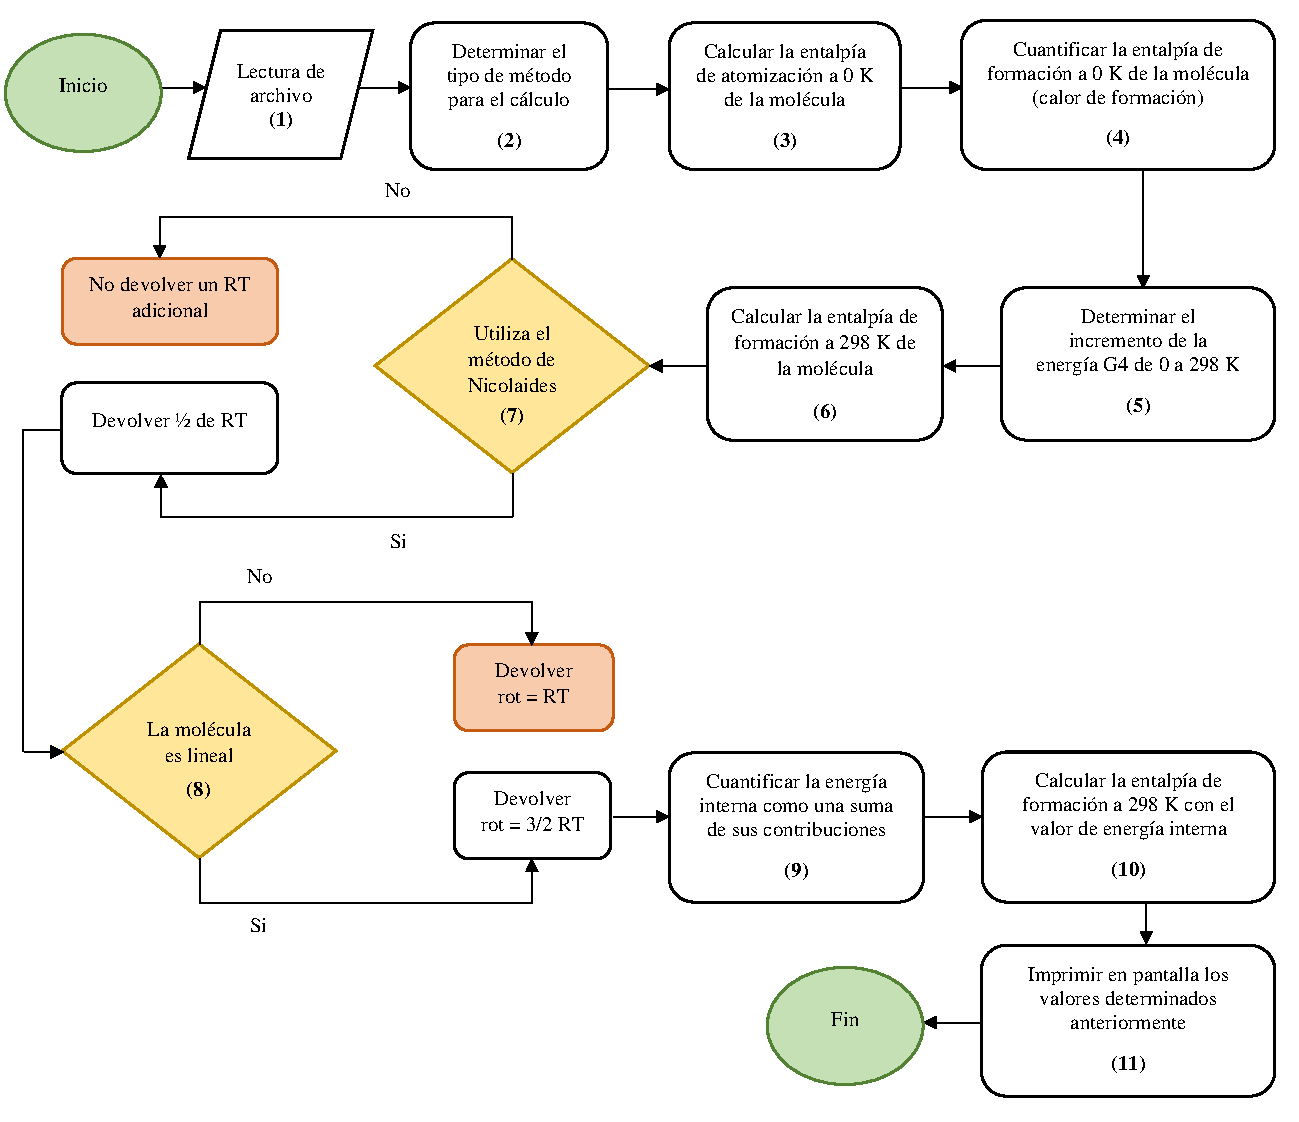
\includegraphics[width=\textwidth]{graphs/diagrama-flujo}
\caption{Diagrama de flujo general}
\label{diagrama-flujo}
\end{center}
\end{figure}


\begin{figure}[hbtp]
\begin{center}
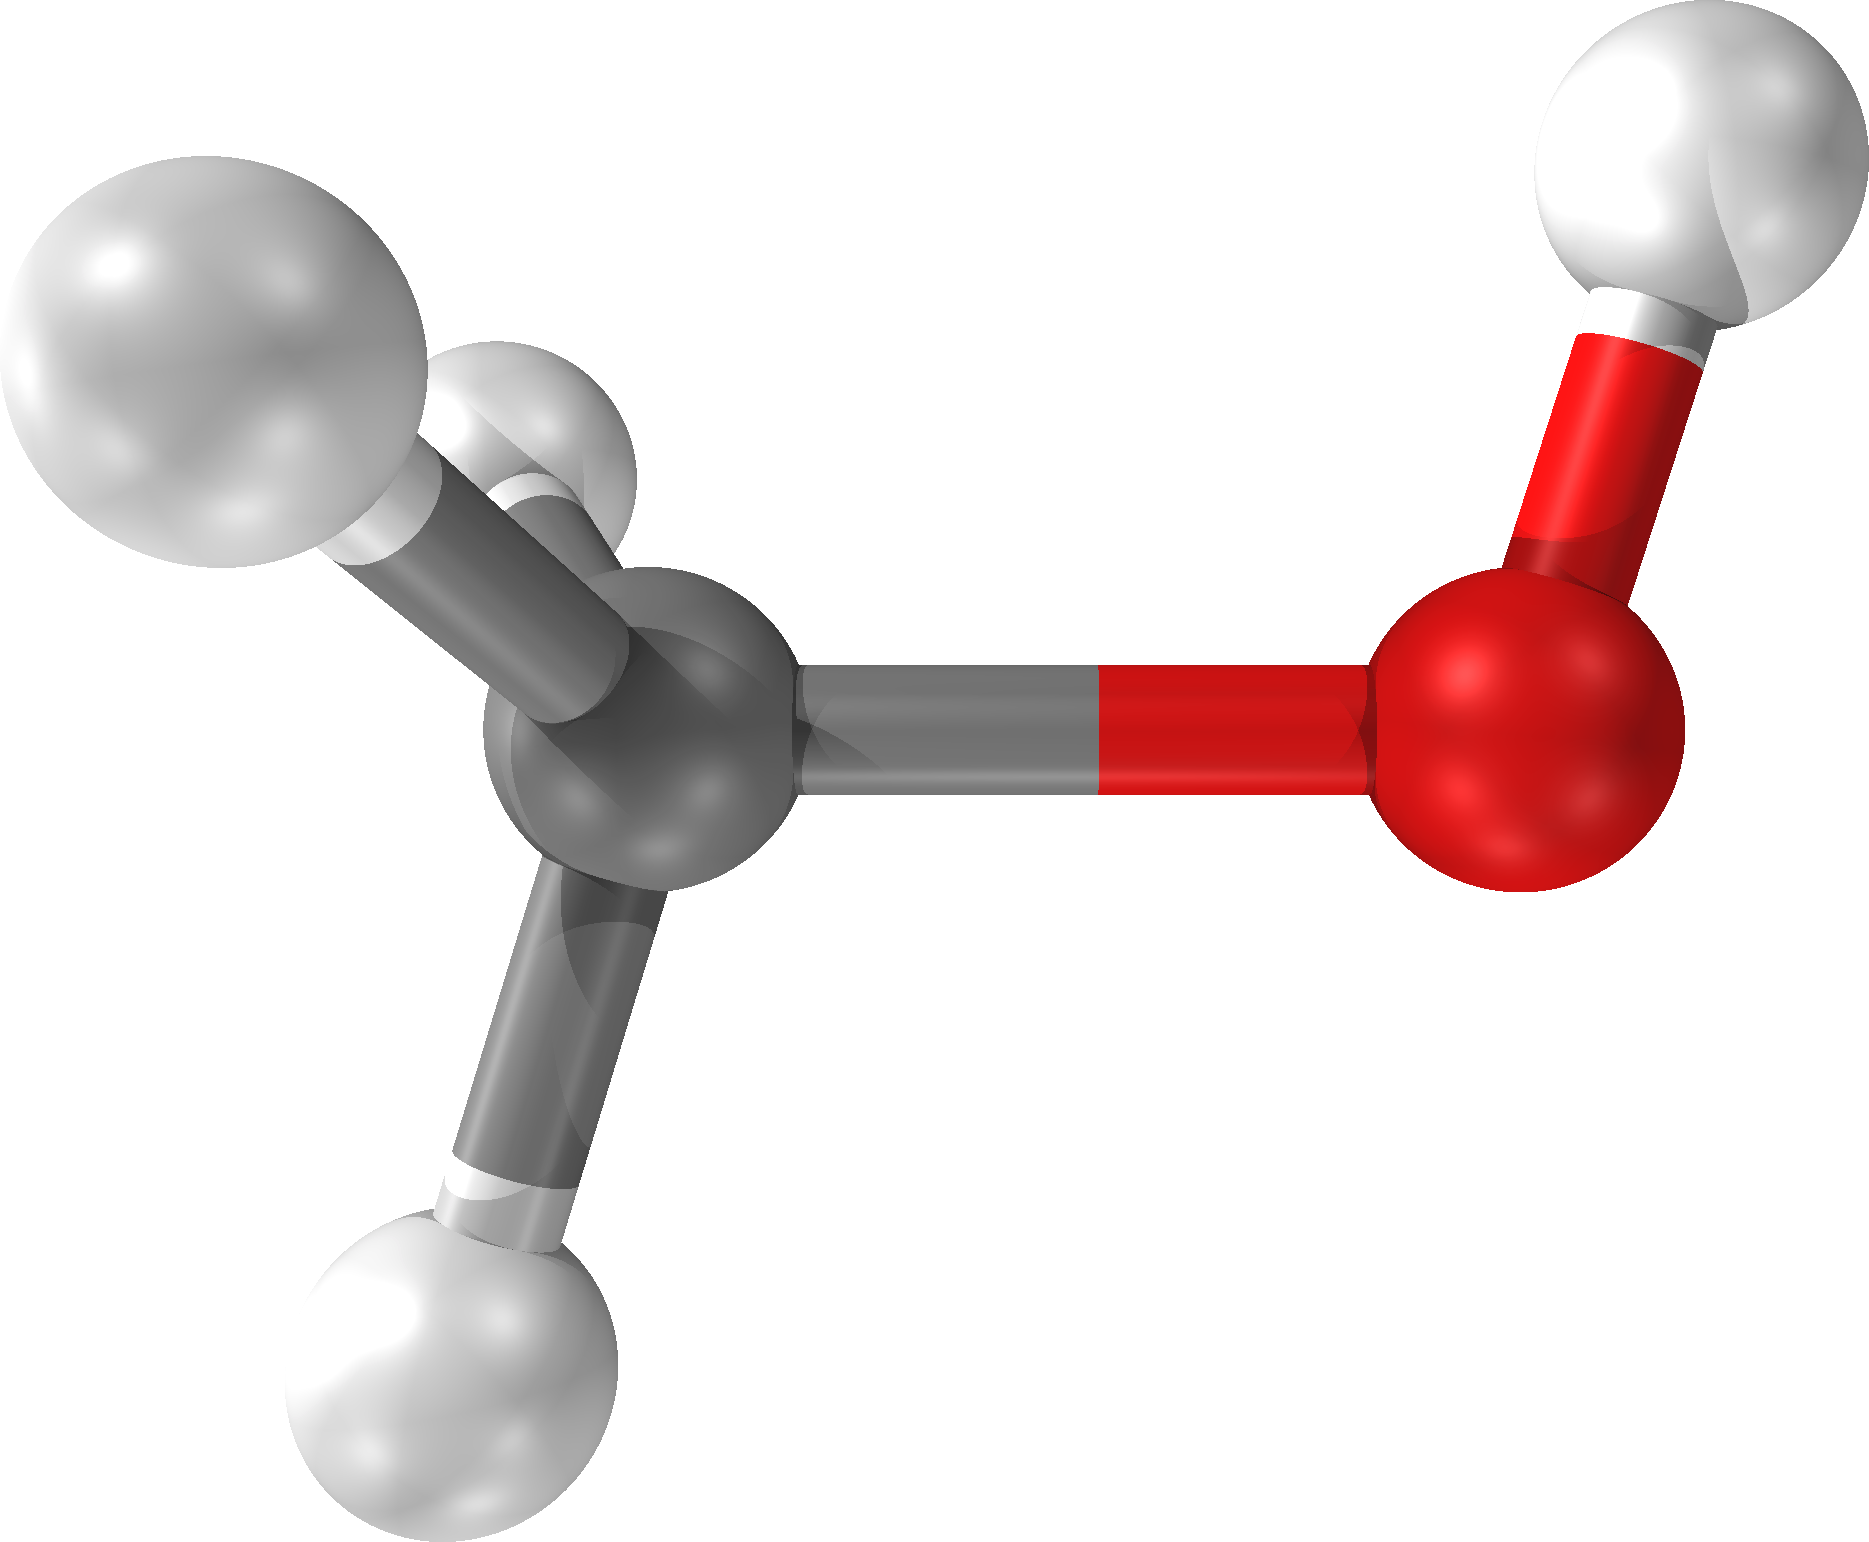
\includegraphics[scale=0.1]{graphs/metanol.png}
\caption{Molécula de metanol, utilizada para explicar el diagrama de flujo general.}
\label{metanol}
\end{center}
\end{figure}

\subsection {Inicio}

El programa comienza con la lectura de un archivo de entrada que contiene la información necesaria de la molécula. Para la \textbf{molécula X}, el archivo de entrada tendrá la siguiente forma:

\begin{lstlisting}[caption = Output de CH3OH-G4.txt]
G4
3
-115.651767
-115.647489
1 4
6 1
8 1
0
0
12
322.7598
1058.0227
1094.4693
1175.9092
1389.4710
1487.0775
1495.0437
1513.5228
2980.0300
3023.9572
3106.3296
3831.1143
\end{lstlisting}



\subsection{Paso 1 del diagrama de flujo general}

Ahora, se leerá el archivo de entrada de la siguiente forma:
\begin{multicols}{2}
\begin{enumerate}		
	\item Categoría de método. 
	\item Número de especies atómicas.
	\item Energía G4 a 0 K.
	\item Entalpía G4 a 0 K.
	\item Número atómico y número de átomos.
	\item Tipo de molécula (lineal o no lineal).
	\item Modelo de aproximación usada (Nicolaides o Rotor Rígido/Oscilador Armónico).
	\item Número de modos de vibración.
	\item Frecuencias vibracionales de la molécula.
\end{enumerate}
\end{multicols}

Las líneas 1, 2, 3, 4 y 5 siempre se encargarán de leer la categoría del método, el número de especies atómicas, la energía G4 a $T$ = 0, la entalpía G4 a $T$ = 0, el número atómico y el número de átomos, respectivamente. Mientras que las líneas 6, 7, 8 y 9 no siempre ocuparán el mismo lugar, porque éstas dependen de líneas anteriores.\\

\newpage

Por ejemplo, para la \textbf{molécula X}, el número de especies atómicas serán tres: Hidrógeno, Carbono y Oxígeno. En consecuencia, la línea 5 se repetirá tres veces para las especies mencionadas. Después, se leerá el tipo de molécula (lineal o no lineal), posteriormente, el modelo de aproximación usada (Nicolaides o Rotor Rígido/Oscilador Armónico). Por último, el número de modos de vibración que influirá en las frecuencias vibracionales de la molécula. Al terminar el proceso de lectura, toda esta información es almacenada en variables específicas del programa. 

 
\subsection{Paso 2 del diagrama de flujo general}

Como tercer paso en el diagrama general, se encuentra la determinación del método utilizado, que es indispensable para comenzar con los cálculos. \textbf{EnthalpyNIST} (uno de los 3 programas creados) cuenta con varios métodos de Gaussian, pero en nuestra explicación utilizaremos sólo el método \textbf{G4 de Gaussian09} (véase el apéndice B para obtener información sobre otros métodos de Gaussian). Hecho esto, el programa tiene la certeza de qué datos ocupar para las especies atómicas antes leídas.



\subsection{Paso 3 del diagrama de flujo general}

En este paso se realiza el cálculo de la entalpía de atomización a $T$ = 0 de la molécula. Aquí se utilizan los valores del método G4 para cada uno de los átomos presentes en la \textbf{molécula X}, la cantidad estequiométrica de estos y la entalpía G4 de la molécula a $T$ = 0 (véase las ecuaciones \ref{eq:4.1} y \ref{eq:4.2}). Para concluir, se realiza una conversión de unidades de energía (hartree a kJ). Obsérvese las ecuaciones \ref{eq:4.4} y \ref{eq:4.5}.

\begin{equation}
	\Delta_\mathrm{{a}} H^{\circleddash}_{\mathrm{0}}\mathrm{(CH_3OH) = \Delta E^\mathrm{{total}}_{0K} (C(^{3}P) + 4H(^{2}S) + O(^{3}S))- \Delta E^\mathrm{{total}}_{0K} (CH_{3}OH)}
\label{eq:4.1}
\end{equation}

\begin{equation}
	\Delta_\mathrm{{a}} H^{\circleddash}_{0}\mathrm{(CH_3OH) = -37.834170\;\mathrm{h} + 4(-0.501420)\;\mathrm{h} - 75.045500\;\mathrm{h} -(-115.651767)\;\mathrm{h}}
\label{eq:4.2}
\end{equation}

\begin{equation}
	\Delta_\mathrm{{a}} H^{\circleddash}_{0}\mathrm{(CH_3OH) = -114.88535\;\mathrm{h} + 115.651767\;\mathrm{h}}
\end{equation}

\begin{equation}
	\Delta_\mathrm{{a}} H^{\circleddash}_{0}\mathrm{(CH_3OH) = (\;0.766417\;\mathrm{h})(2625.4997480\;\mathrm{kJ\;mol^{-1})}}
\label{eq:4.4}
\end{equation}

\begin{equation}
	\Delta_\mathrm{{a}} H^{\circleddash}_{0}\mathrm{(CH_3OH) = 2012.22764\; \mathrm{kJ\;mol^{-1}}}
\label{eq:4.5}
\end{equation}
 
\subsection{Paso 4 del diagrama de flujo general}

En este paso se realiza el cálculo de la entalpía de formación a $T$ = 0 de la molécula. Nuevamente, se utilizan valores experimentales para cada uno de los átomos presentes en la molécula junto con su cantidad específica y el valor de la entalpía de atomización a $T$ = 0 obtenido anteriormente (ecuaciones \ref{eq:4.6} y \ref{eq:4.7}). Al valor obtenido en este paso se le conoce como \textbf{calor de formación} (ecuación \ref{eq:4.9}). Por último, se realiza una conversión de unidades de energía (kJ a kcal), ver las ecuaciones \ref{eq:4.10} y \ref{eq:4.11}. 

\begin{equation}
	\Delta_\mathrm{{f}} H^{\circleddash}_{0}\mathrm{(CH_3OH) = \Delta_{f} H^{\circleddash}_{0}(C(^{3}P) + 4H(^{2}S) + O(^{3}S))- \Delta_{f} H^{\circleddash}_{0} (CH_{3}OH)}
\label{eq:4.6}
\end{equation}

\begin{multline}
	\Delta_\mathrm{{f}} H^{\circleddash}_{0}\mathrm{(CH_3OH)} = 711.185\;\mathrm{kJ\;mol^{-1}} + 4(216.03500)\mathrm{kJ\;mol^{-1}} +...\\
	...\; 246.7900\;\mathrm{kJ\;mol^{-1}} - 2012.22764\; \mathrm{kJ\;mol^{-1}}
\label{eq:4.7}
\end{multline}

\begin{equation}
	\Delta_\mathrm{{f}} H^{\circleddash}_{0}\mathrm{(CH_3OH) = 1822.115 - 2012.22764\; kJ\;mol^{-1}}
\end{equation}

\begin{equation}
	\Delta_\mathrm{{f}} H^{\circleddash}_{0}\mathrm{(CH_3OH) = -190.11264\; kJ\;mol^{-1}}
\label{eq:4.9}
\end{equation}

\begin{equation}
	\Delta_\mathrm{{f}} H^{\circleddash}_{0}\mathrm{(CH_3OH) = (-190.11264\; kJ\;mol^{-1})(0.23888\; kcal)}
\label{eq:4.10}
\end{equation}

\begin{equation}
	\Delta_\mathrm{{f}} H^{\circleddash}_{0}\mathrm{(CH_3OH) = -\;45.41\;kcal}
\label{eq:4.11}
\end{equation}


\subsection{Paso 5 del diagrama de flujo general}

El paso 5 se encarga de cuantificar la diferencia entre las  dos cantidades G4 ($T$ = 0 y $T$ = 298 K) leídas en el paso 1 (ecuación \ref{eq:4.13}). Además, se realiza una conversión de unidades de energía (hartree a kJ), ecuaciones \ref{eq:4.14} y \ref{eq:4.15}.

\begin{equation}
	\Delta \Delta H^{\circleddash}\mathrm{(CH_3OH) = G4\;\textrm{Entalpía} - G4\;(0\;K)}
\label{eq:4.12}
\end{equation}

\begin{equation}
	\Delta \Delta H^{\circleddash}\mathrm{(CH_3OH) = -115.647489\;\mathrm{h} - (-115.651767)\;h}
\label{eq:4.13}
\end{equation}

\begin{equation}
	\Delta \Delta H^{\circleddash}\mathrm{(CH_3OH) = (0.004278\;\mathrm{h})(2625.4997480\; kJ\;mol^{-1})}
\label{eq:4.14}
\end{equation}

\begin{equation}
	\Delta \Delta H^{\circleddash}\mathrm{(CH_3OH) = 11.23188\;kJ\;mol^{-1}}
\label{eq:4.15}
\end{equation}


\subsection{Paso 6 del diagrama de flujo general}

En el paso 6 se obtiene el valor de la entalpía de formación a $T$ = 298 K (sumando el calor de formación, la diferencia de las dos cantidades G4 y restando los incrementos correspondientes para los elementos de la molécula en sus estados estándar), en consecuencia, se usan los valores obtenidos en los pasos 4 y 5 (véase las ecuaciones \ref{eq:4.16}, \ref{eq:4.17}, \ref{eq:4.18} y \ref{eq:4.19}). Finalmente, se realiza una conversión de unidades de energía de kJ a kcal (ecuaciones \ref{eq:4.20} y \ref{eq:4.21}).

\begin{multline}
	\enthalpy*(f){}(CH_3OH) = \Delta_\mathrm{{f}} H^{\circleddash}_{0}\mathrm{(CH_{3}OH)} + \Delta \Delta H^{\circleddash} \mathrm{(CH_{3}OH)} \\ - (\Delta \Delta H^{\circleddash} \mathrm{(C)} + 2 \Delta \Delta H^{\circleddash}\mathrm{(H_{2})} + \frac{1}{2} \Delta \Delta H^{\circleddash}\mathrm{(O_{2}))}
\label{eq:4.16}
\end{multline}

\begin{multline}
	\enthalpy*(f){}\mathrm{(CH_3OH)} = -190.11264\;\mathrm{kJ\;mol^{-1}} + 11.23188\;\mathrm{kJ\;mol^{-1}}  \\ - (1.05100 + 2(8.46700) + \frac{1}{2} (8.67000))\mathrm{\; kJ\;mol^{-1}}
\label{eq:4.17}
\end{multline}

\begin{equation}
	\enthalpy*(f){}\mathrm{(CH_3OH) = -190.11264\;\mathrm{kJ\;mol^{-1}} + 11.23188\;\mathrm{kJ\;mol^{-1}} - 22.3265\;kJ\;mol^{-1}}
\label{eq:4.18}
\end{equation}

\begin{equation}
	\enthalpy*(f){}\mathrm{(CH_3OH) = -201.21\;kJ\;mol^{-1}}
\label{eq:4.19}
\end{equation}

\begin{equation}
	\enthalpy*(f){}\mathrm{(CH_3OH) = (-201.21 kJ\;mol^{-1})(0.23888 \:kcal)}
\label{eq:4.20}
\end{equation}

\begin{equation}
	\enthalpy*(f){}\mathrm{(CH_3OH) = -\;48.06 \:kcal}
\label{eq:4.21}
\end{equation}


\subsection{Paso 7, 8 y 9 del diagrama de flujo general}

Los pasos 7 y 8 son de los más importantes del programa, porque calculan la energía interna (paso 6) usando ecuaciones que provienen de la Termodinámica Estadística. Se inicia con dos sentencias de condición que evalúan parámetros de la molécula, como son:

\begin{multicols}{2}
\begin{enumerate}
	\item Aproximaciones a usar.
	\item El número de modos de vibración.
	\item Frecuencias vibracionales.
	\item Si es lineal o no.
\end{enumerate}
\end{multicols}

El tipo de aproximación usada solo puede tener dos valores, 0 y 1. Si el archivo de entrada de la molécula muestra un valor de 0 significa que se usará la aproximación de Nicolaides \textit{et al.} \cite{Nicolaides1996} (no toma en cuenta las frecuencias vibraciones de la molécula menores a 260 cm$^{-1}$ y devuelve $\frac{1}{2}$ de $RT$ para la contribución vibracional por cada frecuencia que sea menor a 260 cm$^{-1}$). Y si el valor es 1, la aproximación de rotor rígido y oscilador armónico \cite{McQuarrie1976} sera usada para los cálculos. 

También existen dos posibles valores en el archivo de entrada para el parámetro de la linealidad de la molécula. Un valor de 1 devolverá un $RT$ en la contribución rotacional, en cambio, si el valor es 0, el condicional retornará un $\frac{3}{2}$ de $RT$ en la contribución rotacional. Después, se inicia una estructura de control que se repetirá el mismo número de veces que el número de modos de vibración de la molécula (una molécula que tiene $N$ especies atómicas puede tener solamente $3N-6$ modos fundamentales de vibración para una molécula no lineal, o $3N-5$ si la molécula es lineal). \\

La iteración usa las ecuaciones \ref{eq:3.27}, \ref{eq:3.28}, \ref{eq:3.29}, \ref{eq:3.30} y \ref{eq:3.31} que provienen de la Termodinámica Estadística \cite{McQuarrie1976, Irikura1998} ,para determinar a la energía interna como una suma de las contribuciones vibracionales, rotacionales, traslacionales y electrónicas (ecuación \ref{eq:3.31}). La contribuci\'{o}n traslacional siempre tendr\'{a} el valor de $\frac{3}{2} RT$ para cualquier mol\'{e}cula (ecuación \ref{eq:3.27}). Adem\'{a}s, se agrega un $RT$ adicional a la energ\'{i}a interna para convertir la energía en entalpía (el llamado término $pV$, ecuación \ref{eq:3.29}). Cabe aclarar que el valor obtenido en la primera iteración es acumulativo para los subsecuentes. Concluida la determinación, se devuelve la suma total de la energía interna. Para la \textbf{molécula X} el número de modos de vibración será 12 (es una molécula no lineal), por lo consiguiente, la ecuación \ref{eq:3.30} se repetirá 12 veces con cada una de las frecuencias de la molécula. El resultado final es la suma de las contribuciones de la energía interna, véase la ecuación \ref{eq:3.31}.

\begin{multline}
	[H(298.15)-H(0)]= 1315.1747\;\mathrm{kJ\;mol^{-1}} + 3718.4568\;\mathrm{kJ\;mol^{-1}} +...\\...\; 3718.4568\;\mathrm{kJ\;mol^{-1}} + 2478.9712\;\mathrm{kJ\;mol^{-1}} = \mathrm{11.2310\;kJ\;mol^{-1}}
\label{eq:4.22}
\end{multline}

\newpage

\subsection{Paso 10 del diagrama de flujo general}

El paso 10 simplemente remplaza el valor obtenido anteriormente (energía interna), por el valor calculado en el paso 5 en la determinación de la entalpía de formación a $T$ = 298 K, es decir, en el paso 6. Para terminar, se hace una conversión de unidades de energía (kJ a kcal).


\begin{equation}
	\enthalpy*(f){}\mathrm{(CH_3OH) = -190.1126\;\mathrm{kJ\;mol^{-1}} + 11.2310\;\mathrm{kJ\;mol^{-1}} - 22.3265\;kJ\;mol^{-1}}
\label{eq:4.23}
\end{equation}

\begin{equation}
	\enthalpy*(f){}\mathrm{(CH_3OH) = -201.21\;kJ\;mol^{-1}}
\label{eq:4.24}
\end{equation}


\begin{equation}
	\enthalpy*(f){}\mathrm{(CH_3OH) = -\;48.06\;kcal}
\label{eq:4.25}
\end{equation}

\newpage

\subsection{Paso 11 del diagrama de flujo general}
El último paso del diagrama de flujo, se encarga de devolver los valores calculados anteriormente, imprimiéndolos en la pantalla a través de la línea de comandos de la siguiente forma:

\begin{lstlisting}[caption = Output de CH3OH-G4.txt en EnthalpyNIST]
$./computeEnthalpyNIST.x  CH3OH-G4.txt$
========================================================================
          New calculation of molecular enthalpies of formation

      Enthalpies of formation of gaseous atoms at 0 and thermal 
   corrections for elements in their standard state at 298 K from:

            NIST-JANAF Thermochemical Tables J. Physics Chem. 
                    Data Monograph 9, 1998, 1-1951.
========================================================================
Heats of formation:
0K          -190.11 kJ mol-1
0K          -45.41 kcal mol-1

Using Nicolaides method:
298K        -201.21 kJ mol-1
298K        -48.06 kcal mol-1

Using G4: 
298K        -201.21 kJ mol-1
298K        -48.06 kcal mol-1
========================================================================
\end{lstlisting}

\section{Código}
El lenguaje de programación elegido para crear de estos programas es C++. El motivo principal de su uso fue que facilita una programación orientada a objetos que fragmenta el código en partes independientes, permitiendo así, reciclar el código para futuros proyectos \cite{cplusplus2005, Deitel2014, Pitt2017}.

\subsection*{Clases}
Ahora, se enlistan los nombres de las clases utilizadas para estos programas:
\begin{multicols}{2}
\begin{itemize}
	\item Enthalpyinputdata.
	\item Method.
	\item EnthalpyG4.
	\item EnthalpyG3.
	\item EnthalpyG3MP2.
	\item EnthalpyCBS-APNO.
	\item EnthalpyCBS-QB3.
\end{itemize}
\end{multicols}

\subsection*{Clase Enthalpyinputdata}
Enthalpyinputdata se encarga de leer los datos (provenientes de Gaussian) del archivo de entrada. Los datos que lee esta clase son:
\begin{multicols}{2}
\begin{itemize}
	\item Tipo de método.
	\item Número de especies atómicas.
	\item Energía G4 a 0 K.
	\item Entalpía G4 a 0 K.
	\item Número atómico y número de átomos .
	\item Tipo de molécula (lineal o no lineal).
	\item Tipo de aproximación usada (Nicolaides o Rotor Rígido y Oscilador Armónico).
	\item Número de modos de vibración.
	\item Frecuencias vibracionales de la molécula.
\end{itemize}
\end{multicols}
La finalidad de esta clase es determinar y almacenar la información indispensable para comenzar con el cálculo de la entalpía de formación \cite{Pitt2017}. 

\subsection*{Clase Method}
La clase Method se utiliza para seleccionar el tipo de método que se realizó en Gaussian, y así, devolver valores específicos para los átomos de Hidrógeno, Carbono, Oxígeno, Nitrógeno, Flúor y Azufre.

\subsection*{Clases EnthalpyG4 y variantes}
El trabajo de esta clase y sus variantes (EnthalpyG3, EnthalpyG3MP2, EnthalpyCBS-APNO y EnthalpyCBS-QB3) es realizar las operaciones aritméticas para obtener el calor de formación de la molécula, la entalpía de formación a $T$ = 298 K mediante el método de atomización y la entalpía de formación a $T$ = 298 K con correcciones en la energía interna. Para concluir, imprime los resultados a través de la línea de comandos.

\newpage

\section{Conjunto de pruebas}

Como parte del proceso de diseño e implementación  de \textit{software} científico, es fundamental corroborar que los programas funcionan de forma correcta, por lo que se realizaron pruebas con moléculas que cuentan con entalpías de formación conocidas y que han sido reportadas en la literatura científica \cite{Ximello2020}. Las moléculas elegidas son isómeros del nitrobenzaladeído (figura \ref{n-NBA}) y son:

\begin{itemize}
\item 2-nitrobenzaldeh\'{i}do (2NBA).
\item 3-nitrobenzaldeh\'{i}do (3NBA).
\item 4-nitrobenzaldeh\'{i}do (4NBA).
\end{itemize}

Los derivados de nitrobenzaladeh\'{i}do son compuestos aromáticos que tienen un gran número de aplicaciones. Entre ellos se encuentran los intermediarios en la preparación de productos químicos de alto valor agregado, pesticidas, materiales ópticos no lineales, productos farmacéuticos, bases de Schiff, etcétera \cite{Ximello2020}.

\begin{figure}[hbtp]
\begin{center}
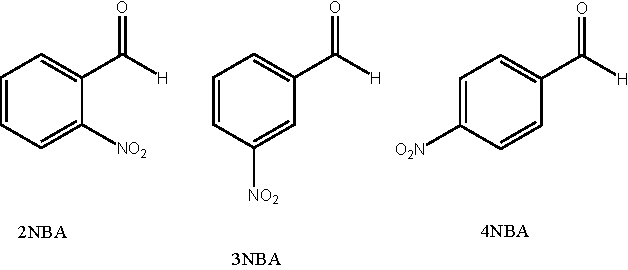
\includegraphics[width=\textwidth]{graphs/n-NBA.pdf}
\caption{Estructuras moleculares de 2-nitrobenzaldeh\'{i}do (2NBA), 3-nitrobenzaldeh\'{i}do (3NBA) y 4-nitrobenzaldeh\'{i}do (4NBA).}
\label{n-NBA}
\end{center}
\end{figure}

Las entalpías de formación de las moléculas fueron calculadas utilizando los métodos G4 y G3MP2, así mismo, se utilizaron las aproximaciones de oscilador armónico/rotor rígido \cite{McQuarrie1976} y Nicolaides \textit{et al.}\cite{Nicolaides1996} en todas las moléculas. Para ello, las frecuencias se calcularon a un nivel teórico B3LYP/6-31G(2df,p) escaladas a 0.9854 y 0.89290. Las entalpías atómicas de formación  fueron a $T$ = 0 y sus correcciones térmicas a $T$ = 298 K se tomaron de la referencia \cite{NIST1998} (excluyendo el valor del átomo de Carbono, cuyo dato coincide con Tajti \textit{et al.} \cite{Tajti2004} para el método G4). Los archivos de salida proceden del \textit{software} \textbf{Gaussian09}, mientras que el archivo que contiene la información necesaria para nuestro programa fue obtenida por el script \textbf{\textit{gendeltahfinputfile}} (proveniente del \textbf{Laboratorio de Fisicoquímica Orgánica Teórica de la BUAP}). Los valores de la entalpía de formación a $T$ = 298 K calculados por nuestro programa del 2-nitrobenzaldehído (2NBA), 3-nitrobenzaldehído (3NBA) y 4-nitrobenzaldehído (4NBA) se muestran a continuación.

\subsection{Conjunto de pruebas: 2NBA, 3NBA y 4NBA}

Es posible apreciar la entalpía de formación a $T$ = 298 K de las 15 simulaciones realizadas en las líneas 22, 20 y 21 de cada molécula, respectivamente. Todos los resultados coinciden con los valores de las moléculas de 2NBA, 3NBA y 4NBA reportados por Ximello \textit{et al.} \cite{Ximello2020}, véase las tablas \ref{Ximello-table-1}, \ref{Ximello-table-2} y \ref{Ximello-table-3}.  

\newpage

%2NBALa-2.txt
\begin{lstlisting}[caption = Output de 2NBALa-2.txt en EnthalpyTajti]
./computeEnthalpyTajti.x 2NBALa-2.txt
========================================================================
           New calculation of molecular enthalpies of formation                         
                                                                                                   
Enthalpies of formation of gaseous atoms at 0 (with the exception of 
carbon data 711.79 kJ/mol from A. Tajti et al. J. Chem. Phys. 121, 
2004, 11599) and thermal corrections for elements in their standard 
states at 298 K from:                   
                                                                                                   
NIST-JANAF Thermochemical Tables J. Physics Chem. Data Monograph 9, 1998,
 1-1951.
========================================================================
Heats of formation:
0K          -8.58 kJ mol-1
0K          -2.05 kcal mol-1

Using Nicolaides method:
298K        -30.82 kJ mol-1
298K        -7.36 kcal mol-1

Using G4 Enthalpy:
298K        -28.19 kJ mol-1
298K        -6.73 kcal mol-1
========================================================================
\end{lstlisting}

\newpage

%2NBALb-2.txt
\begin{lstlisting}[caption = Output de 2NBALb-2.txt en EnthalpyTajti]
./computeEnthalpyTajti.x 2NBALb-2.txt
========================================================================
           New calculation of molecular enthalpies of formation                         
                                                                                                   
Enthalpies of formation of gaseous atoms at 0 (with the exception of 
carbon data 711.79 kJ/mol from A. Tajti et al. J. Chem. Phys. 121, 
2004, 11599) and thermal corrections for elements in their standard 
states at 298 K from:                   
                                                                                                   
NIST-JANAF Thermochemical Tables J. Physics Chem. Data Monograph 9, 1998,
 1-1951.
========================================================================
Heats of formation:
0K          -16.26 kJ mol-1
0K          -3.88 kcal mol-1

Using Nicolaides method:
298K        -38.73 kJ mol-1
298K        -9.25 kcal mol-1

Using G4 Enthalpy:
298K        -36.25 kJ mol-1
298K        -8.66 kcal mol-1
========================================================================
\end{lstlisting}

\newpage

%3NBALa-2.txt
\begin{lstlisting}[caption = Output de 3NBALa-2.txt en EnthalpyTajti]
./computeEnthalpyTajti.x 3NBALa-2.txt
========================================================================
           New calculation of molecular enthalpies of formation                         
                                                                                                   
Enthalpies of formation of gaseous atoms at 0 (with the exception of 
carbon data 711.79 kJ/mol from A. Tajti et al. J. Chem. Phys. 121, 
2004, 11599) and thermal corrections for elements in their standard 
states at 298 K from:                   
                                                                                                   
NIST-JANAF Thermochemical Tables J. Physics Chem. Data Monograph 9, 1998,
 1-1951.
========================================================================
Heats of formation: 
0K          -35.36 kJ mol-1
0K          -8.45 kcal mol-1
                                                                                                   
Using Nicolaides method: 
298K        -57.82 kJ mol-1
298K        -13.81 kcal mol-1
                                                                                                   
Using G4 Enthalpy: 
298K        -55.46 kJ mol-1
298K        -13.25 kcal mol-1
========================================================================
\end{lstlisting}

\newpage

%3NBALb-2.txt
\begin{lstlisting}[caption = Output de 3NBALb-2.txt en EnthalpyTajti]
./computeEnthalpyTajti.x 3NBALb-2.txt
========================================================================
           New calculation of molecular enthalpies of formation                         
                                                                                                   
Enthalpies of formation of gaseous atoms at 0 (with the exception of 
carbon data 711.79 kJ/mol from A. Tajti et al. J. Chem. Phys. 121, 
2004, 11599) and thermal corrections for elements in their standard 
states at 298 K from:                   
                                                                                                   
NIST-JANAF Thermochemical Tables J. Physics Chem. Data Monograph 9, 1998,
 1-1951.
========================================================================
Heats of formation: 
0K          -33.75 kJ mol-1
0K          -8.06 kcal mol-1
                                                                                                   
Using Nicolaides method: 
298K        -56.26 kJ mol-1
298K        -13.44 kcal mol-1
                                                                                                   
Using G4 Enthalpy: 
298K        -53.82 kJ mol-1
298K        -12.85 kcal mol-1
========================================================================
\end{lstlisting}

\newpage

%4NBALa-2.txt
\begin{lstlisting}[caption = Output de 4NBALa-2.txt en EnthalpyTajti]
./computeEnthalpyTajti.x 4NBALa-2.txt
========================================================================
           New calculation of molecular enthalpies of formation                         
                                                                                                   
Enthalpies of formation of gaseous atoms at 0 (with the exception of 
carbon data 711.79 kJ/mol from A. Tajti et al. J. Chem. Phys. 121, 
2004, 11599) and thermal corrections for elements in their standard 
states at 298 K from:                   
                                                                                                   
NIST-JANAF Thermochemical Tables J. Physics Chem. Data Monograph 9, 1998,
 1-1951.
========================================================================
Heats of formation: 
0K          -33.82 kJ mol-1
0K          -8.08 kcal mol-1
                                                                                                   
Using Nicolaides method: 
298K        -56.33 kJ mol-1
298K        -13.45 kcal mol-1
                                                                                                   
Using G4 Enthalpy: 
298K        -53.84 kJ mol-1
298K        -12.86 kcal mol-1
========================================================================
\end{lstlisting}

%%%%%%%%%%%%%%%%%%%%%%%%%%%%%%%%%%%%%%%%%%1%%%%%%%%%%%%%%%%%%%%%%%%%%%%%%%%%%%%%%%%%%%%%%%%%%%%%%%%%%

\newpage

%2NBALa-2.txt
\begin{lstlisting}[caption = Output de 2NBALa-2.txt en EnthalpyNIST]
./computeEnthalpyNIST.x 2NBALa-2.txt
========================================================================
          New calculation of molecular enthalpies of formation

      Enthalpies of formation of gaseous atoms at 0 and thermal 
   corrections for elements in their standard state at 298 K from:

            NIST-JANAF Thermochemical Tables J. Physics Chem. 
                    Data Monograph 9, 1998, 1-1951.
========================================================================
Heats of formation:
0K          -16.61 kJ mol-1
0K          -3.97 kcal mol-1

Using Nicolaides method:
298K        -38.91 kJ mol-1
298K        -9.29 kcal mol-1

Using G3MP2 Enthalpy:
298K        -36.42 kJ mol-1
298K        -8.70 kcal mol-1
========================================================================
\end{lstlisting}

\newpage

%2NBALb-2.txt
\begin{lstlisting}[caption = Output de 2NBALb-2.txt en EnthalpyNIST]
./computeEnthalpyNIST.x 2NBALb-2.txt
========================================================================
          New calculation of molecular enthalpies of formation

      Enthalpies of formation of gaseous atoms at 0 and thermal 
   corrections for elements in their standard state at 298 K from:

            NIST-JANAF Thermochemical Tables J. Physics Chem. 
                    Data Monograph 9, 1998, 1-1951.
========================================================================
Heats of formation:
0K          -7.11 kJ mol-1
0K          -1.70 kcal mol-1

Using Nicolaides method:
298K        -29.28 kJ mol-1
298K        -6.99 kcal mol-1

Using G3MP2 Enthalpy:
298K        -26.60 kJ mol-1
298K        -6.35 kcal mol-1
========================================================================
\end{lstlisting}

\newpage

%3NBALa-2.txt
\begin{lstlisting}[caption = Output de 3NBALa-2.txt en EnthalpyNIST]
./computeEnthalpyNIST.x 3NBALa-2.txt
========================================================================
          New calculation of molecular enthalpies of formation

      Enthalpies of formation of gaseous atoms at 0 and thermal 
   corrections for elements in their standard state at 298 K from:

            NIST-JANAF Thermochemical Tables J. Physics Chem. 
                    Data Monograph 9, 1998, 1-1951.
========================================================================
Heats of formation:
0K          -35.18 kJ mol-1
0K          -8.40 kcal mol-1

Using Nicolaides method:
298K        -57.44 kJ mol-1
298K        -13.72 kcal mol-1

Using G3MP2 Enthalpy:
298K        -54.94 kJ mol-1
298K        -13.12 kcal mol-1
========================================================================
\end{lstlisting}

\newpage

%3NBALb-2.txt
\begin{lstlisting}[caption = Output de 3NBALb-2.txt en EnthalpyNIST]
./computeEnthalpyNIST.x 3NBALb-2.txt
========================================================================
          New calculation of molecular enthalpies of formation

      Enthalpies of formation of gaseous atoms at 0 and thermal 
   corrections for elements in their standard state at 298 K from:

            NIST-JANAF Thermochemical Tables J. Physics Chem. 
                    Data Monograph 9, 1998, 1-1951.
========================================================================
Heats of formation:
0K          -33.44 kJ mol-1
0K          -7.99 kcal mol-1

Using Nicolaides method:
298K        -55.77 kJ mol-1
298K        -13.32 kcal mol-1

Using G3MP2 Enthalpy:
298K        -53.19 kJ mol-1
298K        -12.70 kcal mol-1
========================================================================
\end{lstlisting}

\newpage

%4NBALa-2.txt
\begin{lstlisting}[caption = Output de 4NBALa-2.txt en EnthalpyNIST]
./computeEnthalpyNIST.x 4NBALa-2.txt
========================================================================
          New calculation of molecular enthalpies of formation

      Enthalpies of formation of gaseous atoms at 0 and thermal 
   corrections for elements in their standard state at 298 K from:

            NIST-JANAF Thermochemical Tables J. Physics Chem. 
                    Data Monograph 9, 1998, 1-1951.
========================================================================
Heats of formation:
0K          -33.23 kJ mol-1
0K          -7.94 kcal mol-1

Using Nicolaides method:
298K        -55.54 kJ mol-1
298K        -13.27 kcal mol-1

Using G3MP2 Enthalpy:
298K        -52.91 kJ mol-1
298K        -12.64 kcal mol-1
========================================================================
\end{lstlisting}

%%%%%%%%%%%%%%%%%%%%%%%%%%%%%%%%%%%%%%%%%%%%%%%%%%%%%%%%2%%%%%%%%%%%%%%%%%%%%%%%%%%%%%%%%%%%%%%%%%%%%%%%%%%%%%%%%%%%%%%%%%

\newpage

%2NBALa-2.txt
\begin{lstlisting}[caption = Output de 2NBALa-2.txt en EnthalpyArgonne]
./computeEnthalpyArgonne.x 2NBALa-2.txt
========================================================================
           New calculation of molecular enthalpies of formation                               
                                                                                                   
Enthalpies of formation of gaseous atoms at 0 and thermal corrections 
        for elements in their standard states at 298 K from:
                                                                                                                  
          
                    ARGONNE Thermochemical Tables                                    
                  Warning: sulfur is taken from NIST                                                                                                       
========================================================================
Heats of formation:
0K          -15.20 kJ mol-1
0K          -3.63 kcal mol-1

Using Nicolaides method:
298K        -37.49 kJ mol-1
298K        -8.96 kcal mol-1

Using G3MP2 Enthalpy:
298K        -35.01 kJ mol-1
298K        -8.36 kcal mol-1
========================================================================
\end{lstlisting}

\newpage

%2NBALb-2.txt
\begin{lstlisting}[caption = Output de 2NBALb-2.txt en EnthalpyArgonne]
./computeEnthalpyArgonne.x 2NBALb-2.txt
========================================================================
           New calculation of molecular enthalpies of formation                               
                                                                                                   
Enthalpies of formation of gaseous atoms at 0 and thermal corrections 
        for elements in their standard states at 298 K from:
                                                                                                                  
          
                    ARGONNE Thermochemical Tables                                    
                  Warning: sulfur is taken from NIST                                                                                                       
========================================================================
Heats of formation:
0K          -5.69 kJ mol-1
0K          -1.36 kcal mol-1

Using Nicolaides method:
298K        -27.86 kJ mol-1
298K        -6.65 kcal mol-1

Using G3MP2 Enthalpy:
298K        -25.19 kJ mol-1
298K        -6.02 kcal mol-1
========================================================================
\end{lstlisting}

\newpage

%3NBALa-2.txt
\begin{lstlisting}[caption = Output de 3NBALa-2.txt en EnthalpyArgonne]
./computeEnthalpyArgonne.x 3NBALa-2.txt
========================================================================
           New calculation of molecular enthalpies of formation                               
                                                                                                   
Enthalpies of formation of gaseous atoms at 0 and thermal corrections 
        for elements in their standard states at 298 K from:
                                                                                                                  
          
                    ARGONNE Thermochemical Tables                                    
                  Warning: sulfur is taken from NIST                                                                                                       
========================================================================
Heats of formation:
0K          -33.76 kJ mol-1
0K          -8.06 kcal mol-1

Using Nicolaides method:
298K        -56.02 kJ mol-1
298K        -13.38 kcal mol-1

Using G3MP2 Enthalpy:
298K        -53.52 kJ mol-1
298K        -12.78 kcal mol-1
========================================================================
\end{lstlisting}

\newpage

%3NBALb-2.txt
\begin{lstlisting}[caption = Output de 3NBALb-2.txt en EnthalpyArgonne]
./computeEnthalpyArgonne.x 3NBALb-2.txt
========================================================================
           New calculation of molecular enthalpies of formation                               
                                                                                                   
Enthalpies of formation of gaseous atoms at 0 and thermal corrections 
        for elements in their standard states at 298 K from:
                                                                                                                  
          
                    ARGONNE Thermochemical Tables                                    
                  Warning: sulfur is taken from NIST                                                                                                       
========================================================================
Heats of formation:
0K          -32.03 kJ mol-1
0K          -7.65 kcal mol-1

Using Nicolaides method:
298K        -54.35 kJ mol-1
298K        -12.98 kcal mol-1

Using G3MP2 Enthalpy:
298K        -51.78 kJ mol-1
298K        -12.37 kcal mol-1
========================================================================
\end{lstlisting}

\newpage

%4NBALa-2.txt
\begin{lstlisting}[caption = Output de 4NBALa-2.txt en EnthalpyArgonne]
./computeEnthalpyArgonne.x 4NBALa-2.txt
========================================================================
           New calculation of molecular enthalpies of formation                               
                                                                                                   
Enthalpies of formation of gaseous atoms at 0 and thermal corrections 
        for elements in their standard states at 298 K from:
                                                                                                                  
          
                    ARGONNE Thermochemical Tables                                    
                  Warning: sulfur is taken from NIST                                                                                                       
========================================================================
Heats of formation:
0K          -31.82 kJ mol-1
0K          -7.60 kcal mol-1

Using Nicolaides method:
298K        -54.12 kJ mol-1
298K        -12.93 kcal mol-1

Using G3MP2 Enthalpy:
298K        -51.50 kJ mol-1
298K        -12.30 kcal mol-1
========================================================================
\end{lstlisting}

%%%%%%%%%%%%%%%%%%%%%%%%%%%%%%%%%%%%%%%%%%%%%%%%%%%%%%%%%%%%%%%%%3%%%%%%%%%%%%%%%%%%%%%%%%%%%%%%%%%%%%%

%%%%%%%%%%%%%%%%%%%%%%%%%%%%%%%%%%%%%%%%%%%%%%%%%%%%%%%%%%%3%%%%%%%%%%%%%%%%%%%%%%%%%%%%%%%%%%%%%%%%%%%

\begin{table}[H]
\centering
\begin{tabular}{|c|c|c|}
\hline
	\multicolumn{3}{||c||}{$\enthalpy*(f){}(298.15 \mathrm{K})\; \mathrm{kJ\;mol^{-1}}$}\\
\hline
\hline
	n-NBA & Ximello \textit{et al.} \cite{Ximello2020} & EnthalpyTajti\\ 
\hline 
2NBAa & -28.19 & -28.19\\
\hline
2NBAb & -36.25 & -36.25\\ 
\hline 
3NBAa & -53.82 & -53.82\\
\hline
3NBAb & -55.46 & -55.46\\ 
\hline 
4NBAa & -53.84 & -53.84\\ 
\hline  
\end{tabular} 
	\caption[Entalpías de formación en fase gaseosa obtenidas mediante el método G4 de Gaussian de 2NBA, 3NBA y 4NBA a $T$ = 298 K y $p^{\circ}$ = 0.1 MPa, reportadas por Ximello \textit{et al.} \cite{Ximello2020}.] {Entalpías de formación en fase gaseosa obtenidas mediante el método G4 de Gaussian de 2NBA, 3NBA y 4NBA a $T$ = 298 K y $p^{\circ}$ = 0.1 MPa, reportadas por Ximello \textit{et al.} \cite{Ximello2020}. Obsérvese la segunda columna. Entalpías de formación en fase gaseosa obtenida por nuestro programa EnthalpyTajti, véase la tercer columna.}
\label{Ximello-table-1}
\end{table}

\begin{table}[H]
\centering
\begin{tabular}{|c|c|c|}
\hline
	\multicolumn{3}{||c||}{$\enthalpy*(f){}(298.15 \mathrm{K})\; \mathrm{kJ\;mol^{-1}}$}\\
\hline
\hline
	n-NBA & Ximello \textit{et al.} \cite{Ximello2020} & EnthalpyNIST\\ 
\hline 
2NBAa & -36.42 & -36.42\\
\hline
2NBAb & -26.60 & -26.60\\ 
\hline 
3NBAa & -54.94 & -54.94\\
\hline
3NBAb & -53.19 & -53.19\\ 
\hline 
4NBAa & -52.91 & -52.91\\ 
\hline  
\end{tabular} 
	\caption[Entalpías de formación en fase gaseosa obtenidas mediante el método G3MP2 de Gaussian de 2NBA, 3NBA y 4NBA a $T$ = 298 K y $p^{\circ}$ = 0.1 MPa, reportadas por Ximello \textit{et al.} \cite{Ximello2020}.] {Entalpías de formación en fase gaseosa obtenidas mediante el método G3MP2 de Gaussian de 2NBA, 3NBA y 4NBA a $T$ = 298 K y $p^{\circ}$ = 0.1 MPa, reportadas por Ximello \textit{et al.} \cite{Ximello2020}. Obsérvese la segunda columna. Entalpías de formación en fase gaseosa obtenida por nuestro programa EnthalpyNIST, véase la tercer columna.}
\label{Ximello-table-2}
\end{table}

\begin{table}[H]
\centering
\begin{tabular}{|c|c|c|}
\hline
	\multicolumn{3}{||c||}{$\enthalpy*(f){}(298.15 \mathrm{K})\; \mathrm{kJ\;mol^{-1}}$}\\
\hline
\hline
	n-NBA & Ximello \textit{et al.} \cite{Ximello2020} & EnthalpyArgonne\\ 
\hline
2NBAa & -35.01 & -35.01\\
\hline
2NBAb & -25.19 & -25.19\\ 
\hline 
3NBAa & -53.52 & -53.52\\
\hline
3NBAb & -51.78 & -51.78\\ 
\hline
4NBAa & -51.50 & -51.50\\ 
\hline  
\end{tabular} 
	\caption[Entalpías de formación en fase gaseosa obtenidas mediante el método G3MP2 de Gaussian de 2NBA, 3NBA y 4NBA a $T$ = 298 K y $p^{\circ}$ = 0.1 MPa, reportadas por Ximello \textit{et al.} \cite{Ximello2020}.]{Entalpías de formación en fase gaseosa obtenidas mediante el método G3MP2 de Gaussian de 2NBA, 3NBA y 4NBA a $T$ = 298 K y $p^{\circ}$ = 0.1 MPa, reportadas por Ximello \textit{et al.} \cite{Ximello2020}. Obsérvese la segunda columna. Entalpías de formación en fase gaseosa obtenida por nuestro programa EnthalpyArgonne, véase la tercer columna.}
\label{Ximello-table-3}
\end{table}

\newpage

Una de las razones para utilizar los valores de Tajti \textit{et al.} \cite{Tajti2004} es porque se subraya una ventaja relativa respecto al uso de una reacción elemental, específicamente en compuestos de referencia cuya entalpía de formación es cero por definición porque en cálculos extremadamente precisos evita errores asociados con las entalpías atómicas de formación para especies como el carbono o el flúor. Sin embargo, dado que no es posible hacer un cálculo de calor en un trozo de grafito, se propone un enfoque alternativo. Una de las referencias usadas fue el monóxido de carbono, su elección se debe a su entalpía de formación determinada experimentalmente (-113.81 $\pm$ 0.17 $\;\mathrm{kJ\;mol^{-1}}$ proveniente de las tablas termoquímicas de Rusic \textit{et al.} \cite{Ruscic2005}), esto no esta ligado hacía el átomo de carbono, por lo tanto, debería ser una referencia relativamente estable. Dado que los valores de CO y O ($\enthalpy*(f){}= 246.86 \pm 0.002\;\mathrm{kJ\;mol^{-1}}$), las energías de reacción elementales, deben ajustarse en 360.65 kJ mol$^{-1}$ por cada átomo de carbono para obtener entalpías de formación. Además los resultados que obtuvieron son sorprendentes, para los compuestos que tienen entalpías de formación bien establecidas y consistentes, según lo determinado por el enfoque ATcT de Ruscic \textit{et al.}\cite{Ruscic2005} los valores de calor determinados por el segundo método están dentro de 1 kJ mol$^{-1}$ en todos los casos. La asombrosa precisión de las entalpías de formación de los compuestos bien caracterizados en \cite{Tajti2004} sugiere que son mejores estimaciones que las que se encuentran en la base de datos NIST-JANAF \cite{NIST1998} para todos los compuestos restantes, excepto quizás el amoníaco.\\

Las 15 pruebas preliminares también se realizaron con el fin de reconocer posibles errores en los resultados durante la ejecución de los programas \textbf{EnthalpyTajti}, \textbf{EnthalpyNIST} y \textbf{EnthalpyArgonne}. No obstante, lo anterior sirve para confirmar que las comparación con Ximello \textit{et al.} \cite{Ximello2020} arroja datos con un alto nivel de precisión. Por esta razón, podemos ratificar la utilidad de nuestro programa para realizar cálculos que requieran un alto nivel de confiabilidad en los resultados teóricos. 











\chapter{Conclusión}

El trabajo realizado cumplió con el objetivo principal, es decir la creación de tres programas de cómputo científico que calculan entalpías de formación de compuestos orgánicos a \textit{T} = 298.15 K con correcciones opcionales a la energía interna utilizando aproximaciones como Nicolaides \textit{et al.}, rotor rígido y oscilador armónico, empleando archivos de salida de Gaussian09. Además, se activaron otros métodos con un alto nivel de teoría y conjuntos de bases pequeñas, los cuales fueron: G3, G3MP2, CBS-APNO, CBS-QB3 y G4. De igual forma, se añadieron valores experimentales reportados por la comunidad científica: Tajti \textit{et al.}, NIST y Argonne.\\

También, se lograron otros objetivos específicos:

\begin{itemize}
\item Los programas fueron diseñados para utilizarse a través de la línea de comandos en un sistema operativo de GNU/Linux, dando como resultado, una alta eficiencia en el flujo de trabajo.

\item Se implementó una programación orientada a objetos que fragmentó el código en partes independientes, permitiendo así, reciclar el código para proyectos futuros.
\end{itemize}






% EMPIEZAN LOS APENDICES
\appendix
\chapter{Funcionamiento del programa}


Para comenzar con el uso de los programas es necesario compilar el código. La herramienta de \textbf{Linux} que genera el ejecutable y otros archivos fuente y no fuente se conoce como \textbf{make}. Una vez hecho esto, se produce el ejecutable.
\begin{lstlisting}
$computeEnthalpyNIST.x$
\end{lstlisting}

El funcionamiento adecuado de \textbf{EnthalpyNIST} se muestra a continuación.

\begin{lstlisting}[caption = Output de CH3OH-G4.txt en EnthalpyNIST]
$./computeEnthalpyNIST.x  CH3OH-G4.txt$
========================================================================
          New calculation of molecular enthalpies of formation

      Enthalpies of formation of gaseous atoms at 0 K and thermal 
   corrections for elements in their standard state at 298 K from:

            NIST-JANAF Thermochemical Tables J. Physics Chem. 
                    Data Monograph 9, 1998, 1-1951.
========================================================================
Heats of formation:
0K          -190.11 kJ mol-1
0K          -45.41 kcal mol-1

Using Nicolaides method:
298K        -201.21 kJ mol-1
298K        -48.06 kcal mol-1

Using G4: 
298K        -201.21 kJ mol-1
298K        -48.06 kcal mol-1
========================================================================
\end{lstlisting}

El código desarrollado para este programa puede ser mejorado incorporando las siguientes actualizaciones. 

\subsection*{Restricciones de ejecución}
Para evitar una ejecución del programa de manera indefinida, es oportuno incorporar diferentes mensajes de error, que permitan al usuario identificar un posible problema. Los mensajes tendrían (o tienen) que ver con los siguientes escenarios.
\begin{itemize}
	\item Ingresar un archivo que no contenga la información necesaria.
	\item Cuando no es posible leer el archivo de entrada.
	\item Si el archivo de entrada no cuenta con un formato determinado.
\end{itemize}

\subsection*{Banderas de entrada}
 Incorporar banderas de entrada al código del programa permitirá tener distintas opciones en el cálculo de la entalpía de formación.  Las opciones son necesarias porque calcularían el valor de la entalpía de formación por distintos métodos y valores. Éstas, podrían ser mostradas al usar la bandera “-h”. Las banderas pueden ser utilizadas de la siguiente manera:
\begin{lstlisting}
$./computeEnthalpyNIST.x -h$
\end{lstlisting}
Por lo tanto, la nomeclatura del programa sería:
\begin{lstlisting}
$./computeEnthalpyNIST.x -flag  molecule.txt/.dat$
\end{lstlisting}
Dónde \textbf{molecule.txt o molecule.dat} es el archivo de entrada y \textbf{-flag} es la bandera de entrada que contiene las diferentes opciones para modificar el cálculo. Las banderas pueden ser las siguientes:
\begin{lstlisting}
$-t$
\end{lstlisting}
Utilizar el valor experimental del átomo de Carbono reportado por Tajti \textit{et al.}\cite{Tajti2004}.
\begin{lstlisting}
$-a$
\end{lstlisting}
Activar las tablas termoquímicas del Laboratorio Nacional de Argonne.
\begin{lstlisting}
$-s$ 
\end{lstlisting}
Guardar el archivo de salida. 
\begin{lstlisting}
$-h$ 
\end{lstlisting}
Muestra un menú de ayuda para el manejo del programa. 

\chapter{Programas adicionales}

Además del programa \textbf{EnthalpyNIST}, se crearon 2 programas que permiten determinar la entalpía de formación por distintos métodos al G4 de \textbf{Guassian09}, con diferentes valores reportados en la literatura científica \cite{Simmie2015,NIST1998,Tajti2004}. Sus usos e interfaces son semejantes a \textbf{EnthalpyNIST}, por consiguiente, existe la posibilidad de incorporar nuevos métodos a dichos programas. Los siguientes hipervínculos contienen por separado, los 3 repositorios de los programas creados en este trabajo.\\

\begin{itemize}

	\item \url{https://github.com/Edgargj/EnthalpyNIST}\\
	\item \url{https://github.com/Edgargj/EnthalpyTajti}\\
	\item \url{https://github.com/Edgargj/EnthalpyArgonne}\\

\end{itemize}

\newpage

\section{EnthalpyNIST}

\textbf{EnthalpyNIST} es un programa de cómputo científico que calcula entalpías de formación de átomos en estado gaseoso a  $T$ = 0 con correcciones térmicas para elementos en su estado estándar a $T$ = 298 K \cite{NIST1998,Nicolaides1996,McQuarrie1976}. \textbf{EnthalpyNIST} admite los siguientes métodos de \textbf{Gaussian}: G3, G3MP2, CBS-APNO, CBS-QB3 y G4. \cite{Simmie2015}.

\section{EnthalpyTajti}

\textbf{EnthalpyTajti} es un programa de cómputo científico que calcula entalpías de formación de átomos en estado gaseoso a  $T$ = 0, a excepción de los datos del átomo de Carbono, reportados por Tajti \textit{et al.} \cite{Tajti2004} con correcciones térmicas para elementos en su estado estándar a $T$ = 298 K \cite{NIST1998,Nicolaides1996,McQuarrie1976}. \textbf{EnthalpyTajti} admite los siguientes métodos de \textbf{Gaussian}: G3, G3MP2, CBS-APNO, CBS-QB3 y G4 \cite{Simmie2015}.

\section{EnthalpyArgonne}

\textbf{EnthalpyArgonne} es un programa de cómputo científico que determina entalpías de formación de átomos en estado gaseoso a $T$ = 0 con correcciones térmicas para elementos en su estado estándar a $T$ = 298 K \cite{Nicolaides1996,McQuarrie1976}. Por otra parte, utiliza tablas termoquímicas del Laboratorio Nacional de Argonne (ANL), no obstante, los valores del átomo de Azufre fueron tomados del Insituto Nacional de Estándares y Tecnología (NIST) \cite{NIST1998}. \textbf{EnthalpyArgonne }admite los siguientes métodos de \textbf{Gaussian}: G3, G3MP2, CBS-APNO, CBS-QB3 y G4 \cite{Simmie2015}.

\backmatter
% AQUÍ VA LA BIBLIOGRAFÍA
\markright{Referencias}
\addcontentsline{toc}{chapter}{Referencias}
\renewcommand{\bibname}{Referencias}
\bibliographystyle{bib/general.bst}
\bibliography{bib/listado2.bib}
%\bibliography{listado2.bib}
%TERMINA DOCUMENTO
\end{document}

